\documentclass[12pt, twoside, openright]{report} %fuente a 12pt, formato doble pagina y chapter a la derecha
\raggedbottom % No ajustar el contenido con un salto de pagina

% MÁRGENES: 2,5 cm sup. e inf.; 3 cm izdo. y dcho.
\usepackage[
a4paper,
vmargin=2.5cm,
hmargin=3cm
]{geometry}

% INTERLINEADO: Estrecho (6 ptos./interlineado 1,15) o Moderado (6 ptos./interlineado 1,5)
\renewcommand{\baselinestretch}{1.15}
\parskip=6pt

% DEFINICIÓN DE COLORES para portada y listados de código
\usepackage[table]{xcolor}
\definecolor{azulUC3M}{RGB}{0,0,102}
\definecolor{gray97}{gray}{.97}
\definecolor{gray75}{gray}{.75}
\definecolor{gray45}{gray}{.45}

% Soporte para GENERAR PDF/A
\usepackage[a-1b]{pdfx}

% ENLACES
\usepackage{hyperref}
\hypersetup{colorlinks=true,
	linkcolor=black, % enlaces a partes del documento (p.e. índice) en color negro
	urlcolor=blue} % enlaces a recursos fuera del documento en azul

% Añadir pdfs como partes del documento
\usepackage{pdfpages}

% Quitar la indentación de principio de los parrafos
\setlength{\parindent}{0em}

% EXPRESIONES MATEMATICAS
\usepackage{amsmath,amssymb,amsfonts,amsthm}

\usepackage{txfonts} 
\usepackage[T1]{fontenc}
\usepackage[utf8]{inputenc}

% Insertar graficas y fotos
\usepackage{tikz}
\usepackage{pgfplots}

\usepackage[spanish, es-tabla]{babel} 
\usepackage[babel, spanish=spanish]{csquotes}
\AtBeginEnvironment{quote}{\small}

% diseño de PIE DE PÁGINA
\usepackage{fancyhdr}
\pagestyle{fancy}
\fancyhf{}
\renewcommand{\headrulewidth}{0pt}
\fancyfoot[LE,RO]{\thepage}
\fancypagestyle{plain}{\pagestyle{fancy}}

% DISEÑO DE LOS TÍTULOS de las partes del trabajo (capítulos y epígrafes o subcapítulos)
\usepackage{titlesec}
\usepackage{titletoc}
\titleformat{\chapter}[block]
{\large\bfseries\filcenter}
{\thechapter.}
{5pt}
{\MakeUppercase}
{}
\titlespacing{\chapter}{0pt}{0pt}{*3}
\titlecontents{chapter}
[0pt]                                               
{}
{\contentsmargin{0pt}\thecontentslabel.\enspace\uppercase}
{\contentsmargin{0pt}\uppercase}                        
{\titlerule*[.7pc]{.}\contentspage}                 

\titleformat{\section}
{\bfseries}
{\thesection.}
{5pt}
{}
\titlecontents{section}
[5pt]                                               
{}
{\contentsmargin{0pt}\thecontentslabel.\enspace}
{\contentsmargin{0pt}}
{\titlerule*[.7pc]{.}\contentspage}

\titleformat{\subsection}
{\normalsize\bfseries}
{\thesubsection.}
{5pt}
{}
\titlecontents{subsection}
[10pt]                                               
{}
{\contentsmargin{0pt}                          
	\thecontentslabel.\enspace}
{\contentsmargin{0pt}}                        
{\titlerule*[.7pc]{.}\contentspage}  


% DISEÑO DE TABLAS.
\usepackage{multirow} % permite combinar celdas 
\usepackage{caption} % para personalizar el título de tablas y figuras
\usepackage{floatrow} % utilizamos este paquete y sus macros \ttabbox y \ffigbox para alinear los nombres de tablas y figuras de acuerdo con el estilo definido. Para su uso ver archivo de ejemplo 
\usepackage{array} % con este paquete podemos definir en la siguiente línea un nuevo tipo de columna para tablas: ancho personalizado y contenido centrado
\newcolumntype{P}[1]{>{\centering\arraybackslash}p{#1}}
\DeclareCaptionFormat{upper}{#1#2\uppercase{#3}\par}

% Diseño de tabla para ingeniería
\captionsetup[table]{
	format=hang,
	name=Tabla,
	justification=centering,
	labelsep=colon,
	width=.75\linewidth,
	labelfont=small,
	font=small,
}

% DISEÑO DE FIGURAS.
\usepackage{graphicx}
\graphicspath{{img/}} %ruta a la carpeta de imágenes

% Diseño de figuras para ingeniería
\captionsetup[figure]{
	format=hang,
	name=Fig.,
	singlelinecheck=off,
	labelsep=colon,
	labelfont=small,
	font=small		
}

% NOTAS A PIE DE PÁGINA
\usepackage{chngcntr} %para numeración continua de las notas al pie
\counterwithout{footnote}{chapter}

% LISTADOS DE CÓDIGO
% soporte y estilo para listados de código. Más información en https://es.wikibooks.org/wiki/Manual_de_LaTeX/Listados_de_código/Listados_con_listings
\usepackage{listings}

% definimos un estilo de listings
\lstdefinestyle{estilo}{ frame=Ltb,
	framerule=0pt,
	aboveskip=0.5cm,
	framextopmargin=3pt,
	framexbottommargin=3pt,
	framexleftmargin=0.4cm,
	framesep=0pt,
	rulesep=.4pt,
	backgroundcolor=\color{gray97},
	rulesepcolor=\color{black},
	%
	basicstyle=\ttfamily\footnotesize,
	keywordstyle=\bfseries,
	stringstyle=\ttfamily,
	showstringspaces = false,
	commentstyle=\color{gray45},     
	%
	numbers=left,
	numbersep=15pt,
	numberstyle=\tiny,
	numberfirstline = false,
	breaklines=true,
	xleftmargin=\parindent
}

\captionsetup[lstlisting]{font=small, labelsep=period}
% fijamos el estilo a utilizar 
\lstset{style=estilo}
\renewcommand{\lstlistingname}{\uppercase{Código}}

\pgfplotsset{compat=1.17} 
%-------------
%	DOCUMENTO
%-------------

\begin{document}
\pagenumbering{roman} % Se utilizan cifras romanas en la numeración de las páginas previas al cuerpo del trabajo
	
%----------
%	PORTADA
%----------	
\begin{titlepage}
	\begin{sffamily}
	\color{azulUC3M}
	\begin{center}
		\begin{figure}[H] %incluimos el logotipo de la Universidad
			\makebox[\textwidth][c]{
\includegraphics[width=16cm]{Portada_Logo.png}}
		\end{figure}
		\vspace{2.5cm}
		\begin{Large}
			Grado en Ingeniería Informática\\			
			2020-2021\\
			\vspace{2cm}		
			\textsl{Apuntes}\\
			\bigskip
		\end{Large}
		 	{\Huge Ingeniería del Software}\\
		 	\vspace*{0.5cm}
	 		\rule{10.5cm}{0.1mm}\\
			\vspace*{0.9cm}
			{\LARGE Jorge Rodríguez Fraile\footnote{\href{mailto:100405951@alumnos.uc3m.es}{Universidad: 100405951@alumnos.uc3m.es}  |  \href{mailto:jrf1616@gmail.com}{Personal: jrf1616@gmail.com}}}\\ 
			\vspace*{1cm}
	\end{center}
	\vfill
	\color{black}
		
\includegraphics[width=4.2cm]{img/creativecommons.png}\\
		Esta obra se encuentra sujeta a la licencia Creative Commons\\ \textbf{Reconocimiento - No Comercial - Sin Obra Derivada}
	\end{sffamily}
\end{titlepage}

%----------
%	ÍNDICES
%----------	

%--
% Índice general
%-
\tableofcontents
\thispagestyle{fancy}

%--
% Índice de figuras. Si no se incluyen, comenta las líneas siguientes
%-
\listoffigures
\thispagestyle{fancy}

%----------
%	TRABAJO
%----------	

\pagenumbering{arabic} % numeración con múmeros arábigos para el resto de la publicación	


%----------
%	COMENZAR A ESCRIBIR AQUI
%----------	

\chapter{Información}
\section{Profesores}
\begin{quote}
Magistrales: JESÚS MANUEL POZA CARRASCO (jepozac@inf.uc3m.es)

Prácticas: Maria Luisa Arjonilla marjonil@inf.uc3m.es
\end{quote}

\section{Recursos}
\href{https://a16z.com/2011/08/20/why-software-is-eating-the-world/}{Why
  Software Is Eating the World - Andreessen Horowitz}

\href{https://iansommerville.com/software-engineering-book/}{Images and
Opinions}

\href{http://butunclebob.com/ArticleS.UncleBob.PrinciplesOfOod}{ArticleS.UncleBob.PrinciplesOfOod}

\url{https://loufranco.com/wp-content/uploads/2012/11/cheatsheet.pdf}

  Libros de Martin Fowler:
\begin{itemize}
	\item \href{http://martinfowler.com/books/nosql.html}{NoSQL Distilled}

	\item \href{http://martinfowler.com/books/dsl.html}{Domain Specific
	Languages}
  
	\item \href{http://martinfowler.com/books/refactoring.html}{Refactoring}
  
	\item \href{http://martinfowler.com/books/eaa.html}{P of EAA}
  
	\item \href{http://martinfowler.com/books/uml.html}{UML Distilled}
  
	\item \href{http://martinfowler.com/books/refactoringRubyEd.html}{Refactoring
	Ruby Ed.}
  
	\item \href{http://martinfowler.com/books/ap.html}{Analysis Patterns}
  
	\item \href{http://martinfowler.com/books/pxp.html}{Planning XP}
\end{itemize}
 
  
  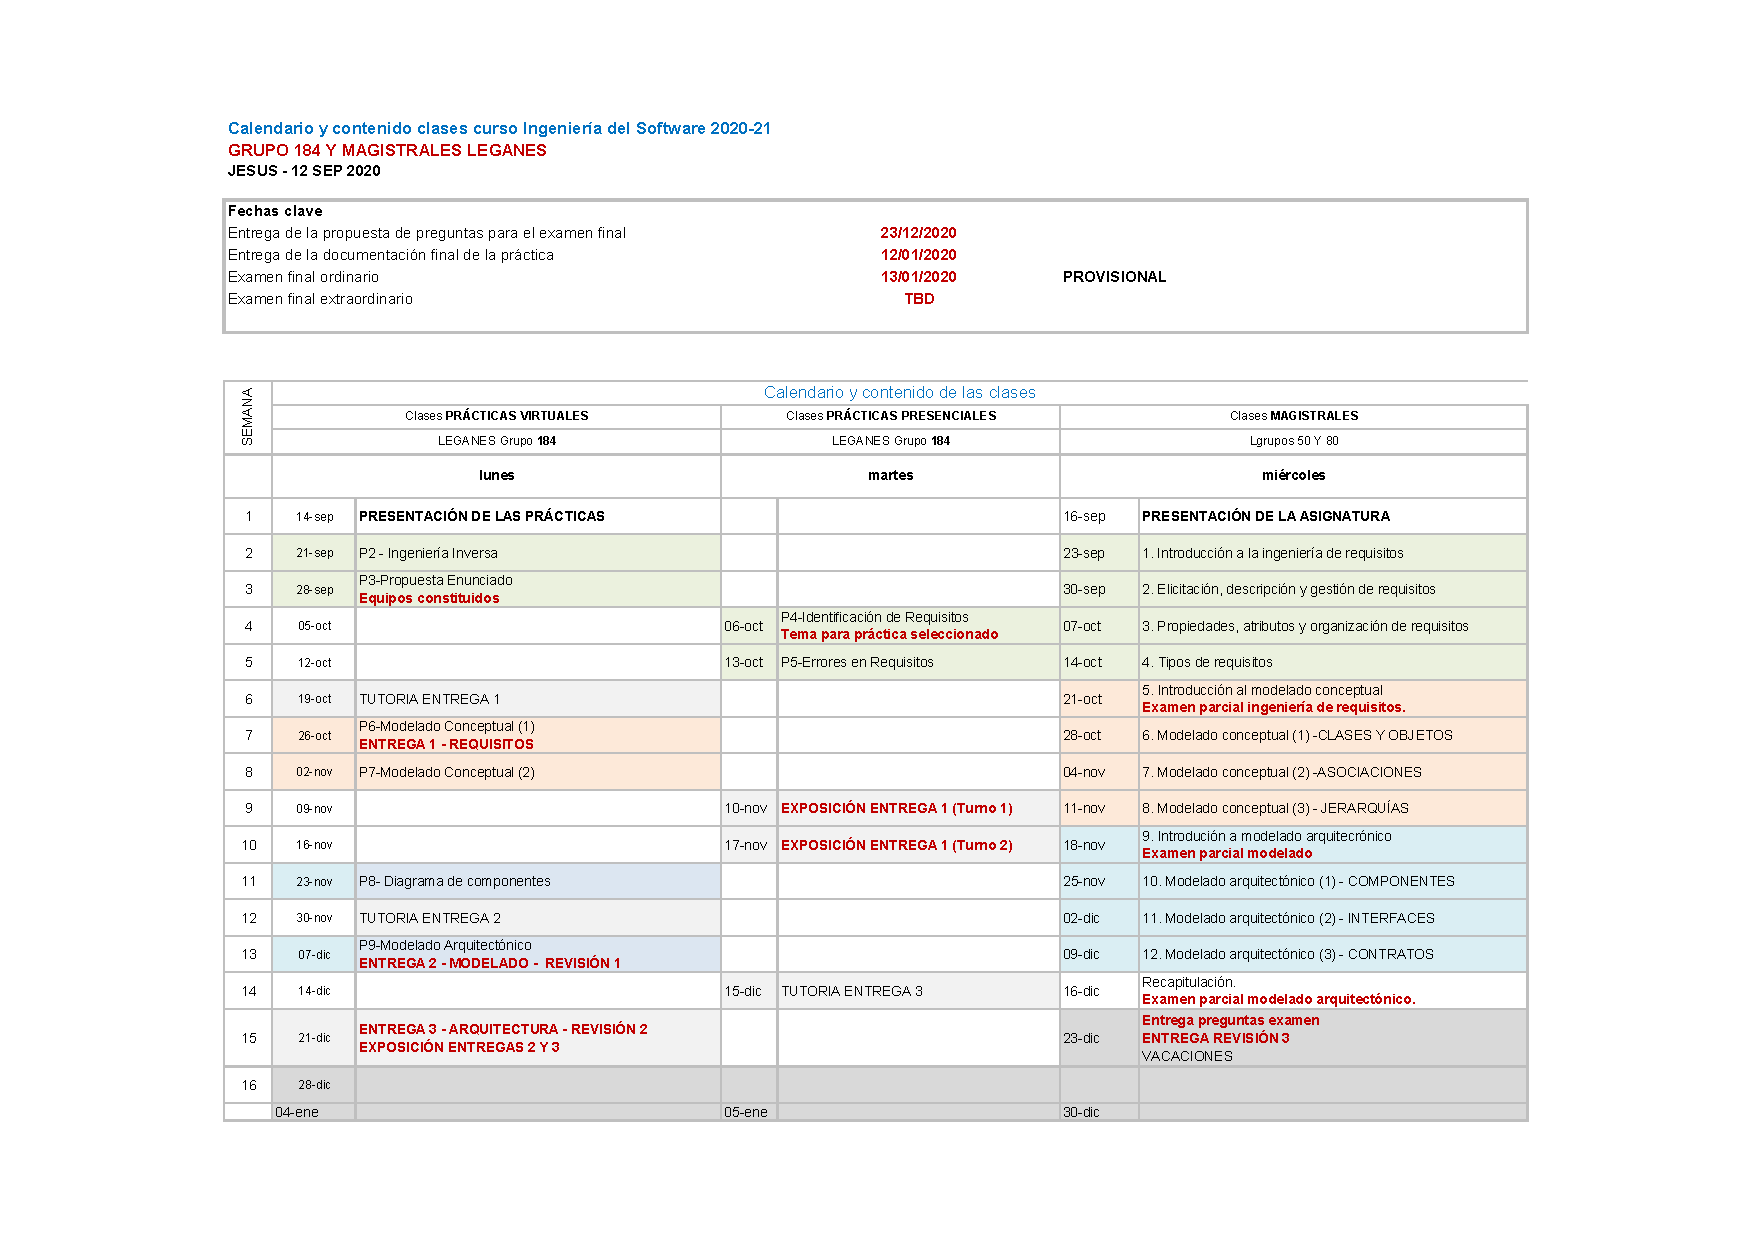
\includepdf[pages=-]{docs/IS_2021_Horario_R_184.pdf}
  
\includepdf[pages=-]{docs/IS_2021_Presentacion_MAGISTRAL.pdf}
  
\part{Teoría}
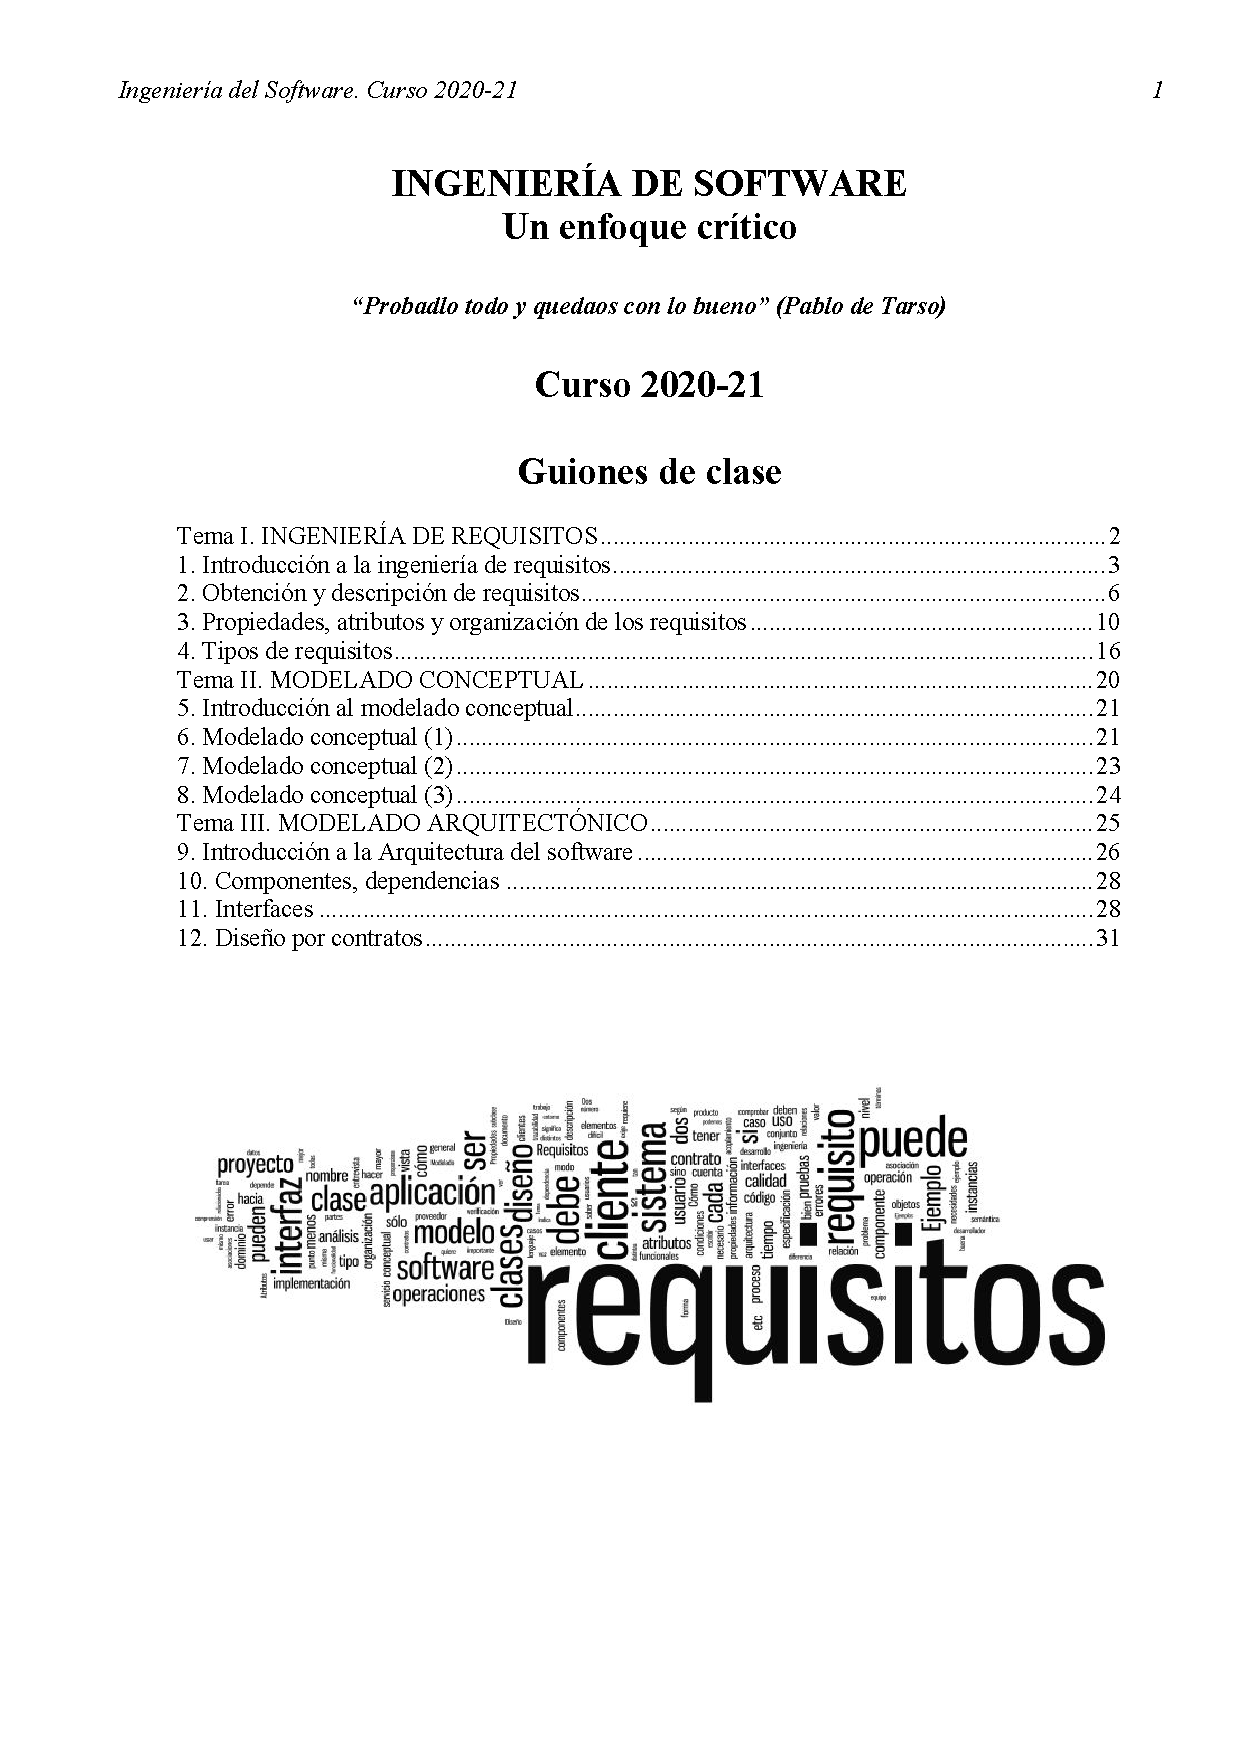
\includepdf[pages=-]{docs/IS_2021_Guiones-Teora.pdf}


\chapter{TEMA 1}

  \url{https://www.barchart.com/stocks/indices/sp-sector/information-technology}

  \url{https://a16z.com/2011/08/20/why-software-is-eating-the-world/}

  \url{https://www.youtube.com/watch?v=8WVoJ6JNLO8\&feature=youtu.be\&ab_channel=RankingTheWorld}

\section{Introducción}

Ingeniería del software: Aplicación sistemática de conocimientos,
métodos y experiencias científicas y tecnológicas al diseño,
implementación, pruebas y documentación de software. Es una
disciplina ubicua, está presente en todo y en todos los tiempos.

Ingeniería de requisitos: Desarrollo sistemático de los requisitos a
través de un proceso iterativo (se repite de forma circular y va
mejorando) y cooperativo en el que se analiza el problema, se
documenta el resultado en diversos formatos de representación, y se
comprueba la exactitud de la comprensión alcanzada.

En ambas disciplinas el producto es software, son más artesanales
que ingenieriles y es necesario describir y documentar lo que se va
a producir.

	
\section{Requisitos}

Lista ordenada de capacidades, funciones, aspectos que debe cumplir el
software que vamos a desarrollar.

\begin{itemize}
  \item
    Condición o capacidad=funcionalidad que el usuario necesita, que
    debe poseer el sistema o aplicación.
  \item
    Estos tienen función contractual en las compañías, para poder exigir
    alcanzar lo acordado.
\end{itemize}
Especificación: Lista de requisitos

Hay que tener en cuenta a todos los interesados o stakeholders,
aquellos que utilizan el sistema. Aunque a veces estos no saben lo
que quieren y por eso se puede volver un proceso complicado.
\pagebreak

Hay estudios que demuestran que la especificación de requisitos es
un factor muy importante para que un proyecto no fracase.

\begin{itemize}

\item
	La nula o mala especificación provoca grandes pérdidas de dinero.
\item
	Aunque tampoco garantiza el éxito.
\end{itemize}

\subsection{Obtención, descripción y escritura de requisitos}

    Tipos:
    \begin{itemize}
		\item
		Requisitos de capacidad (funcionales): Son los de cara al usuario.
		Funciones y operaciones requeridas para resolver un problema o
		alcanzar un objetivo.
		\item
		Requisitos de restricción (no funcionales): Son los relativos a
		las características técnicas, que hacen que el sistema funcione
		aceptablemente. Restricciones impuestas sobre la manera en que el
		problema es resuelto o el objetivo alcanzado.
    \end{itemize}

	V
	\begin{figure}[H]
		\ffigbox[\FBwidth]
		{\caption{V Ingenieria de Software}}
		{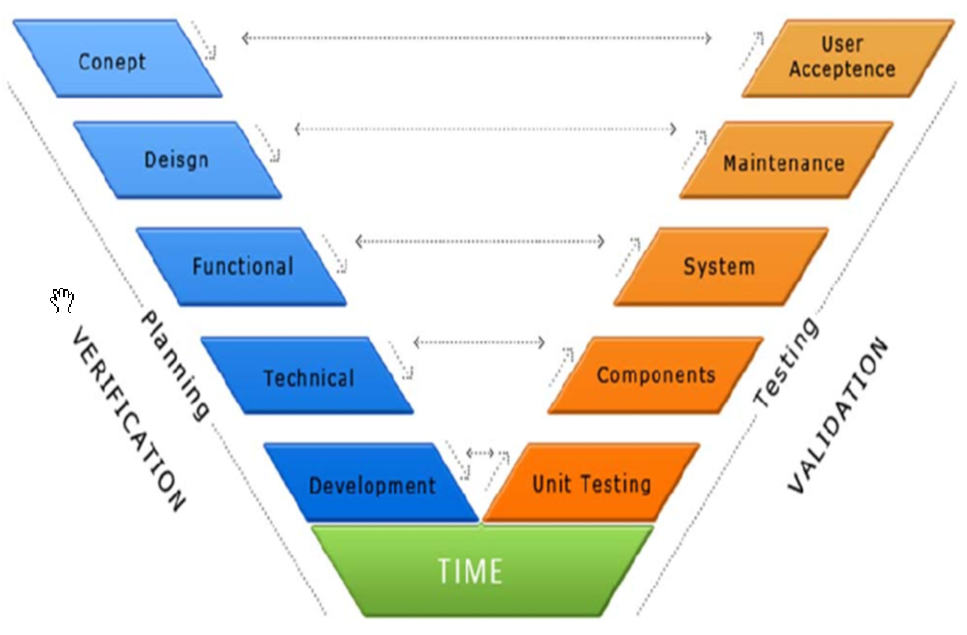
\includegraphics[scale=.3]{Untitled.png}}
	\end{figure}

	Plan para obtener requisitos:
    \begin{itemize}
		\item
		Identificar: Conocer a los stakeholders.
		\item
		Entrevistar: A los stakeholders para recoger requisitos.
		\item
		Escribir: Los requisitos se documentan.
		\item
		Revisar: Analizamos los requisitos, si pasa la revisión seguimos,
		si no volvemos a identificar.
    \end{itemize}

	Técnicas para la obtención y descripción de requisitos.
    \begin{itemize}
		\item
		Textuales: Accesibles a un cliente sin formación específica.
		\begin{itemize}
			\item
				En prosa común y corriente.
			\item
				Texto estructurado, casos de uso o tabla de roles de usuario y
				servicio.
		\end{itemize}
		\item Gráficas: Requieren un cierto grado de formación técnica.
			\begin{itemize}
			\item Con cuidado, no se tienen que convertir en diseño.
					\begin{itemize}
						\item
						Diagramas de flujos de datos.
						\item
						Diagramas de actividad.
						\item
						diagramas de estado.
					\end{itemize}
			\item Interfaces de usuario y prototipos: No confundir con diseño.
			\end{itemize}
	\end{itemize}


	Técnicas de elicitación:

    \begin{itemize}
		\item
		Historias de usuario: Manera cómoda de obtener especificaciones de
		los usuarios. Lo escriben ellos mismos.
			\begin{itemize}
				\item
					Como \_\_\_ quiero \_\_\_\_ para \_\_\_\_
			\end{itemize}
		\item
		Prototipos: Permite extraer requisitos, ensayar soluciones y
		eliminar partes arriesgadas. Se realizan en fases tempranas, para
		que el usuario lo vea y exprese lo que desea y saber si se va por
		buen camino. No tiene que ser funcional más visual, y no tarda
		demasiado.
			\begin{itemize}
				\item Mock-ups (maquetas): Modelo o prototipo.
			\end{itemize}
		\item
		Diagramas de Casos de uso: Muestran las funciones y la relación
		entre los actores y dichas funciones de un sistema.
		\begin{figure}[H]
			\ffigbox[\FBwidth]
			{\caption{Caso de Uso}}
			{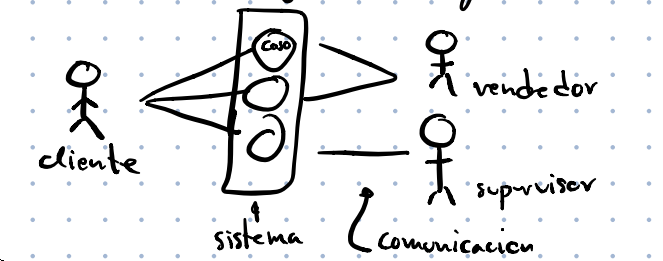
\includegraphics[scale=.3]{Untitled 1.png}}
		\end{figure}
		

    \end{itemize}
 \pagebreak
	Ciclo de vida:
	\begin{figure}[H]
		\ffigbox[\FBwidth]
		{\caption{Ciclo de vida de los requisitos}}
		{

			\tikzset{every picture/.style={line width=0.75pt}} %set default line width to 0.75pt        
			
			\begin{tikzpicture}[x=0.75pt,y=0.75pt,yscale=-1,xscale=1]
			%uncomment if require: \path (0,300); %set diagram left start at 0, and has height of 300
			
			%Straight Lines [id:da5128943707394515] 
			\draw    (90,80) -- (138,80) ;
			\draw [shift={(140,80)}, rotate = 180] [color={rgb, 255:red, 0; green, 0; blue, 0 }  ][line width=0.75]    (10.93,-3.29) .. controls (6.95,-1.4) and (3.31,-0.3) .. (0,0) .. controls (3.31,0.3) and (6.95,1.4) .. (10.93,3.29)   ;
			%Straight Lines [id:da5763174393271724] 
			\draw    (220,80) -- (268,80) ;
			\draw [shift={(270,80)}, rotate = 180] [color={rgb, 255:red, 0; green, 0; blue, 0 }  ][line width=0.75]    (10.93,-3.29) .. controls (6.95,-1.4) and (3.31,-0.3) .. (0,0) .. controls (3.31,0.3) and (6.95,1.4) .. (10.93,3.29)   ;
			%Straight Lines [id:da42693718637793476] 
			\draw    (380,80) -- (438,80) ;
			\draw [shift={(440,80)}, rotate = 180] [color={rgb, 255:red, 0; green, 0; blue, 0 }  ][line width=0.75]    (10.93,-3.29) .. controls (6.95,-1.4) and (3.31,-0.3) .. (0,0) .. controls (3.31,0.3) and (6.95,1.4) .. (10.93,3.29)   ;
			%Straight Lines [id:da2054123248619093] 
			\draw    (530,80) -- (588,80) ;
			\draw [shift={(590,80)}, rotate = 180] [color={rgb, 255:red, 0; green, 0; blue, 0 }  ][line width=0.75]    (10.93,-3.29) .. controls (6.95,-1.4) and (3.31,-0.3) .. (0,0) .. controls (3.31,0.3) and (6.95,1.4) .. (10.93,3.29)   ;
			%Straight Lines [id:da9456140516556879] 
			\draw    (60,120) -- (40,120) -- (40,102) ;
			\draw [shift={(40,100)}, rotate = 450] [color={rgb, 255:red, 0; green, 0; blue, 0 }  ][line width=0.75]    (10.93,-3.29) .. controls (6.95,-1.4) and (3.31,-0.3) .. (0,0) .. controls (3.31,0.3) and (6.95,1.4) .. (10.93,3.29)   ;
			%Straight Lines [id:da34310034992991034] 
			\draw    (210,120) -- (190,120) -- (190,102) ;
			\draw [shift={(190,100)}, rotate = 450] [color={rgb, 255:red, 0; green, 0; blue, 0 }  ][line width=0.75]    (10.93,-3.29) .. controls (6.95,-1.4) and (3.31,-0.3) .. (0,0) .. controls (3.31,0.3) and (6.95,1.4) .. (10.93,3.29)   ;
			%Straight Lines [id:da9018210017852952] 
			\draw    (370,120) -- (350,120) -- (350,102) ;
			\draw [shift={(350,100)}, rotate = 450] [color={rgb, 255:red, 0; green, 0; blue, 0 }  ][line width=0.75]    (10.93,-3.29) .. controls (6.95,-1.4) and (3.31,-0.3) .. (0,0) .. controls (3.31,0.3) and (6.95,1.4) .. (10.93,3.29)   ;
			%Straight Lines [id:da07024328206064778] 
			\draw    (170,100) -- (170,120) -- (152,120) ;
			\draw [shift={(150,120)}, rotate = 360] [color={rgb, 255:red, 0; green, 0; blue, 0 }  ][line width=0.75]    (10.93,-3.29) .. controls (6.95,-1.4) and (3.31,-0.3) .. (0,0) .. controls (3.31,0.3) and (6.95,1.4) .. (10.93,3.29)   ;
			%Straight Lines [id:da5122232045007191] 
			\draw    (300,100) -- (300,120) -- (282,120) ;
			\draw [shift={(280,120)}, rotate = 360] [color={rgb, 255:red, 0; green, 0; blue, 0 }  ][line width=0.75]    (10.93,-3.29) .. controls (6.95,-1.4) and (3.31,-0.3) .. (0,0) .. controls (3.31,0.3) and (6.95,1.4) .. (10.93,3.29)   ;
			%Straight Lines [id:da04657498204663235] 
			\draw    (460,100) -- (460,120) -- (442,120) ;
			\draw [shift={(440,120)}, rotate = 360] [color={rgb, 255:red, 0; green, 0; blue, 0 }  ][line width=0.75]    (10.93,-3.29) .. controls (6.95,-1.4) and (3.31,-0.3) .. (0,0) .. controls (3.31,0.3) and (6.95,1.4) .. (10.93,3.29)   ;
			%Straight Lines [id:da5495934480516471] 
			\draw    (610,100) -- (610,160) -- (542,160) ;
			\draw [shift={(540,160)}, rotate = 360] [color={rgb, 255:red, 0; green, 0; blue, 0 }  ][line width=0.75]    (10.93,-3.29) .. controls (6.95,-1.4) and (3.31,-0.3) .. (0,0) .. controls (3.31,0.3) and (6.95,1.4) .. (10.93,3.29)   ;
			%Straight Lines [id:da7039881630970108] 
			\draw    (630,100) -- (630,180) -- (542,180) ;
			\draw [shift={(540,180)}, rotate = 360] [color={rgb, 255:red, 0; green, 0; blue, 0 }  ][line width=0.75]    (10.93,-3.29) .. controls (6.95,-1.4) and (3.31,-0.3) .. (0,0) .. controls (3.31,0.3) and (6.95,1.4) .. (10.93,3.29)   ;
			%Straight Lines [id:da21922014405830548] 
			\draw    (650,100) -- (650,200) -- (572.6,200.19) ;
			\draw [shift={(570.6,200.2)}, rotate = 359.86] [color={rgb, 255:red, 0; green, 0; blue, 0 }  ][line width=0.75]    (10.93,-3.29) .. controls (6.95,-1.4) and (3.31,-0.3) .. (0,0) .. controls (3.31,0.3) and (6.95,1.4) .. (10.93,3.29)   ;
			%Straight Lines [id:da7271984969396854] 
			\draw    (450,160) -- (330,160) -- (330,102) ;
			\draw [shift={(330,100)}, rotate = 450] [color={rgb, 255:red, 0; green, 0; blue, 0 }  ][line width=0.75]    (10.93,-3.29) .. controls (6.95,-1.4) and (3.31,-0.3) .. (0,0) .. controls (3.31,0.3) and (6.95,1.4) .. (10.93,3.29)   ;
			%Straight Lines [id:da5939873506600859] 
			\draw    (450,180) -- (180,180) -- (180,102) ;
			\draw [shift={(180,100)}, rotate = 450] [color={rgb, 255:red, 0; green, 0; blue, 0 }  ][line width=0.75]    (10.93,-3.29) .. controls (6.95,-1.4) and (3.31,-0.3) .. (0,0) .. controls (3.31,0.3) and (6.95,1.4) .. (10.93,3.29)   ;
			%Straight Lines [id:da8269525689572383] 
			\draw    (430,200) -- (30,200) -- (30,102) ;
			\draw [shift={(30,100)}, rotate = 450] [color={rgb, 255:red, 0; green, 0; blue, 0 }  ][line width=0.75]    (10.93,-3.29) .. controls (6.95,-1.4) and (3.31,-0.3) .. (0,0) .. controls (3.31,0.3) and (6.95,1.4) .. (10.93,3.29)   ;
			
			% Text Node
			\draw    (9,68) -- (84,68) -- (84,93) -- (9,93) -- cycle  ;
			\draw (12,72) node [anchor=north west][inner sep=0.75pt]   [align=left] {Elicitación};
			% Text Node
			\draw    (154,69) -- (213,69) -- (213,94) -- (154,94) -- cycle  ;
			\draw (157,73) node [anchor=north west][inner sep=0.75pt]   [align=left] {Analisis};
			% Text Node
			\draw    (273.54,68) -- (376.54,68) -- (376.54,92) -- (273.54,92) -- cycle  ;
			\draw (276.54,72) node [anchor=north west][inner sep=0.75pt]   [align=left] {Especificación};
			% Text Node
			\draw    (443.07,70) -- (528.07,70) -- (528.07,95) -- (443.07,95) -- cycle  ;
			\draw (446.07,74) node [anchor=north west][inner sep=0.75pt]   [align=left] {Verificación};
			% Text Node
			\draw    (595,69) -- (671,69) -- (671,94) -- (595,94) -- cycle  ;
			\draw (598,73) node [anchor=north west][inner sep=0.75pt]   [align=left] {Validación};
			% Text Node
			\draw (68,111) node [anchor=north west][inner sep=0.75pt]   [align=left] {clasificación};
			% Text Node
			\draw (220,100) node [anchor=north west][inner sep=0.75pt]   [align=left] {\begin{minipage}[lt]{35.62pt}\setlength\topsep{0pt}
			\begin{center}
			cerrar\\huecos
			\end{center}
			
			\end{minipage}};
			% Text Node
			\draw (381,103) node [anchor=north west][inner sep=0.75pt]   [align=left] {\begin{minipage}[lt]{37.87pt}\setlength\topsep{0pt}
			\begin{center}
			arreglar\\errores
			\end{center}
			
			\end{minipage}};
			% Text Node
			\draw (462,151) node [anchor=north west][inner sep=0.75pt]   [align=left] {reescribir};
			% Text Node
			\draw (463,173) node [anchor=north west][inner sep=0.75pt]   [align=left] {reevaluar};
			% Text Node
			\draw (432,191) node [anchor=north west][inner sep=0.75pt]   [align=left] {confirmar y corregir};
			% Text Node
			\draw (4,12) node [anchor=north west][inner sep=0.75pt]   [align=left] {\begin{minipage}[lt]{59.43pt}\setlength\topsep{0pt}
			\begin{center}
			Requisitos\\identificados
			\end{center}
			
			\end{minipage}};
			% Text Node
			\draw (147,12) node [anchor=north west][inner sep=0.75pt]   [align=left] {\begin{minipage}[lt]{50.93pt}\setlength\topsep{0pt}
			\begin{center}
			Requisitos\\depurados
			\end{center}
			
			\end{minipage}};
			% Text Node
			\draw (275.04,12) node [anchor=north west][inner sep=0.75pt]   [align=left] {\begin{minipage}[lt]{69.64pt}\setlength\topsep{0pt}
			\begin{center}
			Requisitos\\documentados
			\end{center}
			
			\end{minipage}};
			% Text Node
			\draw (449.07,12) node [anchor=north west][inner sep=0.75pt]   [align=left] {\begin{minipage}[lt]{51.47pt}\setlength\topsep{0pt}
			\begin{center}
			Requisitos\\verificados
			\end{center}
			
			\end{minipage}};
			% Text Node
			\draw (597,12) node [anchor=north west][inner sep=0.75pt]   [align=left] {\begin{minipage}[lt]{50.35pt}\setlength\topsep{0pt}
			\begin{center}
			Requisitos\\validados
			\end{center}
			
			\end{minipage}};
			
			
			\end{tikzpicture}}
	\end{figure}
    \begin{itemize}
		\item Verificación: Comprobar que funciona tal y como se espera.
			\begin{itemize}
				\item Do the thing right, hacer las cosas
			\end{itemize}
		\item Validación: El usuario/stakeholder está de acuerdo/acepta.
			\begin{itemize}
				\item Do the right thing, hacer la tarea correcta.
			\end{itemize}
    \end{itemize}

	Especificación inteligente de requisitos:
	\begin{itemize}
		\item e\textbf{S}pecifico: Claro y simple.
		\item \textbf{M}edible: Se puede cuantificar y evaluar.
		\item \textbf{A}lineado: Con la estrategia o con el fin del sistema.
		\item \textbf{R}ealista: Puede conseguirse con un numero de recursos lógicos.
		\item limitado en \textbf{T}iempo: Establece un periodo de tiempo.
	\end{itemize}
\pagebreak
\subsection{Como escribir buenos requisitos. Propiedades de los requisitos}



    Una buena especificación es completa, consistente entre requisitos y
    correcta definición de requisitos.

    \begin{itemize}
    
    \item
      Completa: Que no falte ningún requisito, cubra todas las
      necesidades y requisitos del usuario.
    \item
      Consistente: No haya conflicto entre requisitos, ya que hay tantos
      que surgen sin querer.
    \item
      Correcta: Cada requisito por individual sea de la manera que debe
      ser, se entienda, sea adecuado gramaticalmente y ortográficamente.
    \item
      Además:

      \begin{itemize}
      
      \item
        Modificable: Puedan variar con las revisiones.
      \item
        Verificable: Hay una condición que puedo probar y verificar.
      \item
        Trazable: Se puede seguir el proceso llevado, demostrando que
        todo está presente.
      \item
        Claros/No ambiguos: No da lugar a varias interpretaciones.
      \end{itemize}
    \end{itemize}

	Estructura de la especificación:

    \begin{itemize}
    
    \item
      Puede haber centenares de requisitos.
    \item
      Escribir los requisitos para no olvidarlos y además pueden ser
      firmados (pieza clave en contratos), fuente del diseño y se
      verifica el software con ellos.
    \item
      La organización es vital.
    \end{itemize}

	Especificaciones completas:

    \begin{itemize}
    
    \item
      Muchas reuniones con clientes, afectados, expertos, etc. Cruzar
      las revisiones de las distintas reuniones, para conectar todos los
      requisitos.
    \item
      Revisiones por pares.
    \item
      Emplear check-lists de proyectos previos que vamos creando con la
      experiencia, que nos ayuden a no olvidar nada.
    \item
      Reutilizar requisitos de proyectos previos similares.

      \begin{itemize}
      
      \item
        Grano grueso: Componentes reutilizables
      \item
        Grano fino: buscadores avanzados.
      \end{itemize}
    \end{itemize}

	Especificación consistente:

    \begin{itemize}
    
    \item
      Tras escribir los requisitos, buscar contradicciones y
      redundancias, que se solapen o dependan unos de otros.
    \item
      Se usan revisiones en grupo y técnicas automáticas de herramientas
      de apoyo.

      \begin{itemize}
      
      \item
        Comparación de grafos semánticos.
      \item
        Detección de unidades inconsistentes.
      \end{itemize}
    \end{itemize}

	Poner un glosario con términos del dominio y posibles acrónimos
    utilizados.

	La especificación de requisitos no es una novela:

    \begin{itemize}
    
    \item
      Estilo narrativo objetivo, plano. Sin valoraciones, adjetivos o
      adverbios.
    \item
      Textos simples y claros
    \item
      Gramáticas fijas y simples
    \item
      Voz activa
    \item
      Evitar terminología no definida.
    \item
      Requisitos fáciles de medir.
    \item
      Ambigüedad cero.
    \item
      No dar conocimiento por sentado

      \begin{itemize}
      
      \item
        Deben ser autocontenidos.
      \end{itemize}
    \item
      Orden lógico y bien estructurado.
    \item
      Cada requisito debe ser atómico.
    \item
      Escribirse con herramientas especializadas para:

      \begin{itemize}
      
      \item
        Identificarlos unívocamente.
      \item
        Atomizarlos
      \item
        Organizarlos, categorizarlos y relacionarlos.
      \item
        Reutilizarlos por separado o en conjunto.
      \item
        Medir su calidad individual o global.
      \end{itemize}
    \end{itemize}
\pagebreak
	Indicadores de calidad:

    \begin{itemize}
    
    \item
      Tamaño del requisito: El justo, 1 frase o como mucho 2. Medido en
      caracteres, palabras o párrafos.
    \item
      Legibilidad: La máxima posible, evitar referirnos a requisitos
      anteriores.
    \item
      Tiempo verbal: Imperativa en lugar de condicional.
    \item
      Modo verbal: Voz activa.
    \item
      Sentencias opcionales y especulativas: Evitar ``quizá'',
      ``usualmente''\ldots{}
    \item
      Expresiones ambiguas: Evitar expresiones, poner cifras numéricas y
      medibles.
    \item
      Sentencias subjetivas: Evitar incluirse a uno mismo. ``yo
      creo\ldots{}'', ``En mi opinión''
    \item
      Sentencias implícitas: Evitar abuso de los pronombres, siempre que
      se pueda.
    \item
      Conectores: Su abuso indica que se incluye más de una necesidad o
      exceso de detalle.
    \item
      Negaciones: más de una palabra negativa en la misma frase es
      difícil de entender.
    \item
      Sentencias incompletas: Evitar sentencias de tipo: ``etcétera'',
      ``entre otros'', ``\ldots{}''
    \item
      Términos propios de diseño o de flujo: Evitar términos que denotan
      diseño.
    \item
      Numero de términos del dominio: Exceso de términos del dominio del
      contexto puede indicar que se están mezclando diferentes
      necesidades en el mismo requisito.
    \item
      Numero de verbos principales: Verbos los justos y necesarios.
    \item
      Acrónimos y abreviaturas: Solo si están definidos en el documento.
    \item
      Estructura gramatical: Usuario/Acción/Objeto/Cualificador.
    \end{itemize}

	Los siete pecados del especificador:

    \begin{itemize}
    
    \item
      Ruido: Información irrelevante.
    \item
      Silencio: Aspectos no cubiertos.
    \item
      Ambigüedad: Admiten varias interpretaciones.
    \item
      Referencia futura: Definida más adelante, pero si se admiten
      referencias cruzadas entre requisitos.
    \item
      Contradicción; Dos o más formas incompatibles.
    \item
      Sobre especificación: Elementos que no corresponden al problema
      sino a una posible solución.
    \item
      Pensamiento ilusorio: Definir el problema de tal forma que
      imposibilita una solución realista.
    \end{itemize}

	Errores típicos:

    \begin{itemize}
    
    \item
      Modo condicional: Evitarlo, usar presente del indicativo o futuro
      inmediato.
    \item
      Detalles de diseño: Evite detalles demasiado técnicos o del
      diseño.
    \item
      Opcionalidad: Exprese la opcionalidad mediante un atributo del
      requisito, indicarlo directamente.
    \item
      Atomicidad: Dar demasiado detalle, mejor pone un requisito por
      cada necesidad.
    \item
      Acrónimos y vaguedad: Acrónimos cuando estén comúnmente aceptados
      y utilizar medidas físicas, no términos como rápido o amigable.
    \item
      Puntuación y legibilidad: Uso apropiado de puntuación. El número
      de sílabas por palabra y palabras por frase es un indicador de
      legibilidad.
    \item
      Pronombres: El exceso de pronombres puede hacer un requisito
      difícil de entender.
    \item
      Pseudocódigo: Evitar el uso de pseudocódigo y los requisitos
      extensos.
    \item
      Numero de términos: Exceso de términos diferentes en el mismo
      requisito puede indicar mezcla de necesidades o demasiado detalle.
	\item
	  Subjetividad, exceso de negaciones.
	\item
	  Falta de precisión: Evite expresiones vagas.
    \end{itemize}
  \pagebreak
\subsection{Tipos de requisitos. Organización de requisitos. Matrices de trazabilidad}


    Tipos de requisitos del software:

    \begin{itemize}
    \item
      Niveles:

      \begin{itemize}
      
      \item
        Requisitos del usuario: Son aquellos que nos los dicen los
        usuarios.
		\item
		Requisitos del Software: Son las descripciones formales de los
		requisitos de usuario, documentadas. Agregan detalles a la
		especificación.
	

		\item
		  Diferencias:
			\begin{table}[h]
				\begin{tabular}{|c|c|c|}
				\hline
									 & \multicolumn{1}{c|}{\textbf{Requisitos del Usuario}}                                                                                                   & \multicolumn{1}{c|}{\textbf{Requisitos del Software}}                                                                                                           \\ \hline
				\textbf{objetivos}   & \begin{tabular}[c]{@{}c@{}}planteamiento del problema\\ captura de requisitos\end{tabular}                                                             & \begin{tabular}[c]{@{}c@{}}refinamiento del problema\\ análisis de requisitos\end{tabular}                                                                       \\ \hline
				\textbf{fuente}      & usuario/cliente                                                                                                                                        & usuario/cliente y análisis                                                                                                                                      \\ \hline
				\textbf{responsable} & usuario/cliente                                                                                                                                        & analista                                                                                                                                                        \\ \hline
				\textbf{audiencia}   & usuario/cliente (y desarrollador)                                                                                                                      & desarrollador (y usuario/cliente)                                                                                                                               \\ \hline
				\textbf{énfasis}     & \begin{tabular}[c]{@{}c@{}}perspectiva del producto\\ características de los usuarios\\ entorno operacional\\ captura mediante prototipos\end{tabular} & \begin{tabular}[c]{@{}c@{}}conocimiento de expertos\\ modelo, métodos formales\\ organización, no dejar cabos sueltos\\ consistencia y completitud\end{tabular} \\ \hline
				\end{tabular}
				\end{table}
		\end{itemize}
  
    \item
      Clasificación de requisitos:

      \begin{itemize}
      
      \item
        Requisitos funcionales: Que tiene que hacer.
      \item
        Requisito no funcionales: Como lo hace, características
        técnicas y restricciones del cómo.

        \begin{itemize}
        
        \item
          Consumo de recursos: Memoria, capacidad\ldots{}
        \item
          Rendimiento: Velocidad, tiempo de respuesta\ldots{}
        \item
          Fiabilidad y disponibilidad.
        \item
          Manejo de errores: Del entorno e internos.
        \item
          Requisitos de interfaz.
		\item
		  Restricciones.
		\item
		  Seguridad del sistema o de las personas.
        \end{itemize}
      \end{itemize}
    \end{itemize}
\pagebreak
	Métodos para organizar los requisitos del software:

    \begin{itemize}
    
    \item
      Según el modelo del sistema:

      \begin{itemize}
      
      \item
        Según el modelo de casos de uso.
      \item
        Según el modelo conceptual.
      \end{itemize}
    \item
      Ciclo de vida de los requisitos.
    \item
      Uso de herramientas para analizar y organizar requisitos.
    \end{itemize}

  Matrices de trazabilidad: Para ir siguiendo que no se nos pase ningún
  requisito de usuario o documentar para que sea de software. 
  

  \begin{itemize}
  \item  Relaciona un requisito de usuario con aquellos de software que lo
	contienen, y también controlamos lo contrario, no poner algo que no
	nos piden.

	\begin{table}[h]
		\begin{tabular}{|c|c|c|}
		\hline
		\textbf{RU} & \textbf{RS} & \textbf{Unidades de implementación} \\ \hline
		1           & 1, 2        & 1                                   \\ \hline
		2           & 3           & 1, 3                                \\ \hline
		3           & 2, 4, 5     & 2                                   \\ \hline
		\end{tabular}
		\end{table}

  \item
    También puede ser de requisitos y clases, marcando en donde se
    encuadra cada uno. Así se ve si todos tienen clase y no haya clases
    vacías, o requisitos sin asignar.

	\begin{table}[h]
		\begin{tabular}{c|c|c|}
		\cline{2-3}
										  & \textbf{Clase 1} & \textbf{Clase 2} \\ \hline
		\multicolumn{1}{|c|}{\textbf{r1}} &                  & X                \\ \hline
		\multicolumn{1}{|c|}{\textbf{r2}} & X                &                  \\ \hline
		\end{tabular}
		\end{table}

\end{itemize}
	Matriz de referencias cruzadas:

    \begin{itemize}
    
    \item
      Controla:

      \begin{itemize}
      
      \item
        Conflictos: fallos entre requisitos.
    \item
      Acoplamiento: dependencias de las que tenemos que tener cuidado,
      pero no son fallos.
      \item
        Redundancia: Decir lo mismo dos veces, se puede reformular, pero
        no es fallo.
      \end{itemize}
    \end{itemize}

	\begin{table}[h]
		\begin{tabular}{|c|c|c|c|c|c|c|c|}
		\hline
					& \textbf{R1} & \textbf{R2} & \textbf{R3} & \textbf{R4} & \textbf{R5} & \textbf{R6} & \textbf{R6} \\ \hline
		\textbf{R1} &             &             & +           &             & x           & x           &             \\ \hline
		\textbf{R2} &             &             &             &             &             &             &             \\ \hline
		\textbf{R3} & +           &             &             & +           &             & +           &             \\ \hline
		\textbf{R4} &             &             & +           &             & x           &             & o           \\ \hline
		\textbf{R5} & x           &             &             & x           &             &             &             \\ \hline
		\textbf{R6} & x           &             & +           &             &             &             &             \\ \hline
		\textbf{R7} &             &             &             & o           &             &             &             \\ \hline
		\end{tabular}
		\end{table}
		\begin{table}[h]
			\begin{tabular}{|l|l|l|l|}
			\hline
			\textbf{Conflicto (x)}                                              & \textbf{Acoplamiento (+)}                                           & \textbf{Redundancia (o)}                                                       & \textbf{Independiente} \\ \hline
			\begin{tabular}[c]{@{}l@{}}R1 y R5\\ R1 y R6\\ R4 y R5\end{tabular} & \begin{tabular}[c]{@{}l@{}}R1 y R3\\ R3 y R4\\ R3 y R6\end{tabular} & \begin{tabular}[c]{@{}l@{}}R4 y R7\\ (-\textgreater R7xR5, R7+R3)\end{tabular} & R2                     \\ \hline
			\end{tabular}
			\end{table}

\pagebreak
	Ejemplo plantilla de requisito

	\begin{table}[h]
		\begin{tabular}{|l|l|}
		\hline
		\textbf{ID}          & 007                                                                                                                                                                                                                                                              \\ \hline
		\textbf{Título}      & Usuarios Visitantes                                                                                                                                                                                                                                              \\ \hline
		\textbf{Tipo}        & Funcional                                                                                                                                                                                                                                                        \\ \hline
		\textbf{Descripción} & \begin{tabular}[c]{@{}l@{}}Los usuarios Visitantes no son usuarios registrados del sistema: pueden\\ acceder libremente a las funciones del rol Visitante sin necesidad de\\ registrarse ni de iniciar sesión, y sin límite de sesiones simultáneas\end{tabular} \\ \hline
		\textbf{Pruebas}     & \begin{tabular}[c]{@{}l@{}}1. Comprobar que para todas las funciones del rol Visitante el sistema\\ no requiere inicio de sesión.\\ \\ 2. Comprobar que el número de sesiones simultáneas de usuarios\\ Visitantes es limitado.\end{tabular}                     \\ \hline
		\end{tabular}
		\end{table}

	Propiedades y atributos deseables de los requisitos del software.

    \begin{itemize}
    
    \item
      Completitud, organización por tipos de requisitos. Matriz de
      trazabilidad.
    \item
      Consistencia, matriz de referencias cruzadas.
    \item
      Corrección, tamaño adecuado, claridad, capacidad de comprobación y
      condiciones de error.
    \end{itemize}

\chapter{TEMA 2 - Modelado}


    Modelo: Abstracción o simplificación de una realidad compleja.
    Representar realidades. Contar historias.

    \begin{itemize}
    
    \item
      Tipos:

      \begin{itemize}
      
      \item
        Modelos formales: Funcionan más como un mensaje. Lenguaje
        universal, precisión, rigor.
      \item
        Modelos informales: Sin lenguaje común.
      \end{itemize}
    \item
      El lenguaje es vehículo del pensamiento.
    \item
      Elemento esencial del proceso de desarrollo de software.
    \item
      Requiere un lenguaje adecuado.
    \end{itemize}

	Modelar es pensar con diagramas.

	Propiedades deseables:

    \begin{itemize}
    
    \item
      Comprensible: Se pueda entender fácilmente.
    \item
      Preciso: Representación fiel del sistema.
    \item
      Predictivo: Se puede utilizar para obtener conclusiones sobre el
      sistema.
    \item
      Barato: más económico que construir y estudiar el sistema.
    \end{itemize}

	Sistema: Colección de elementos organizados para cumplir una
    finalidad.

	Modelo: Abstracción de un sistema, una simplificación para
    comprenderlo mejor.

	Diagrama: Representación gráfica de un conjunto de elementos
    interconectados.

	Componentes de un lenguaje:

    \begin{itemize}
    
    \item
      Fonología.
    \item
      Semántica.
    \item
      Gramática.
    \item
      Pragmática.
    \end{itemize}

	UML - Unified Modeling Language: Es un lenguaje de modelado.

	Tipos de Diagramas:

    \begin{itemize}
    
    \item
      Los más importantes:

      \begin{itemize}
      \item
        Casos de Uso: Muestra la relación de los actores con el sistema
        y lo que este le ofrece al user. Sirve para especificar la
        comunicación.
		\begin{figure}[H]
			\ffigbox[\FBwidth]
			{\caption{Casos de Uso}}
			{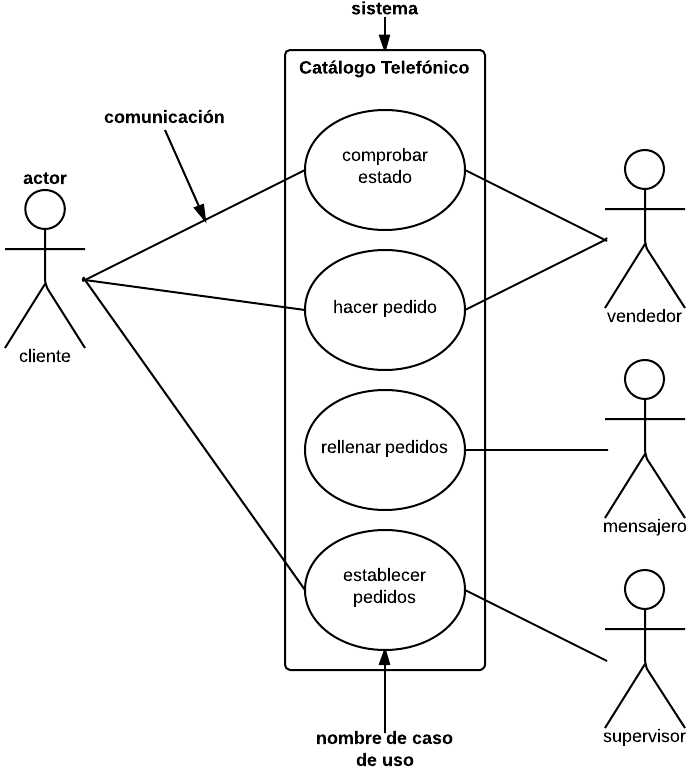
\includegraphics[scale=.3]{Untitled 9.png}}
		\end{figure}
      \item
        De clases: Muestra las clases de nuestro sistema como
        sustantivos, con sus atributos y operaciones, y conectan con los
        relacionados.
		\begin{figure}[H]
			\ffigbox[\FBwidth]
			{\caption{Diagrama de Clases}}
			{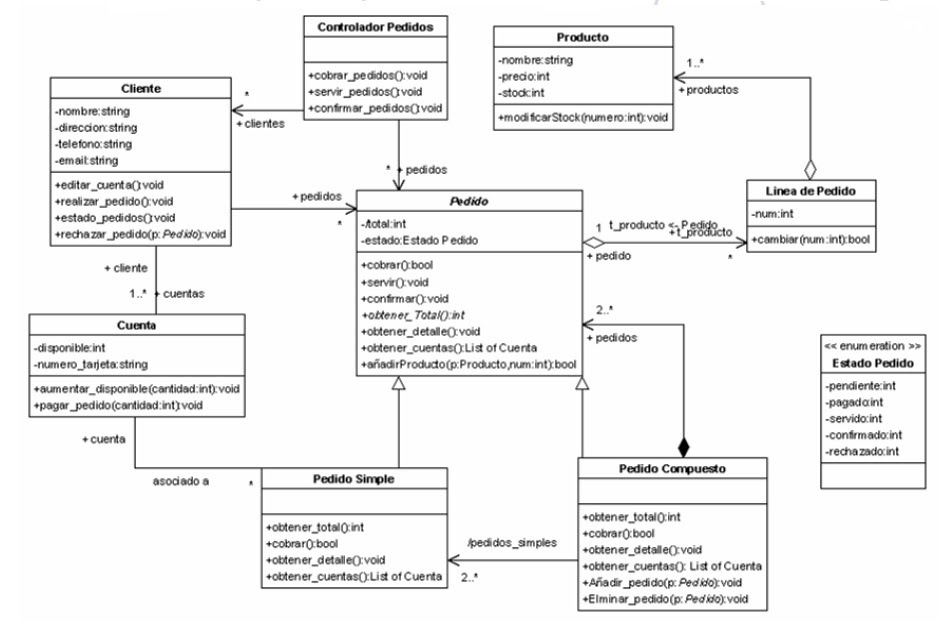
\includegraphics[scale=.3]{Untitled 10.png}}
		\end{figure}
		\pagebreak
      \item
        De componentes: Representa como un sistema de software es
        dividido en componentes y muestra las dependencias entre los
        componentes.
		\begin{figure}[H]
			\ffigbox[\FBwidth]
			{\caption{Diagrama de Componentes}}
			{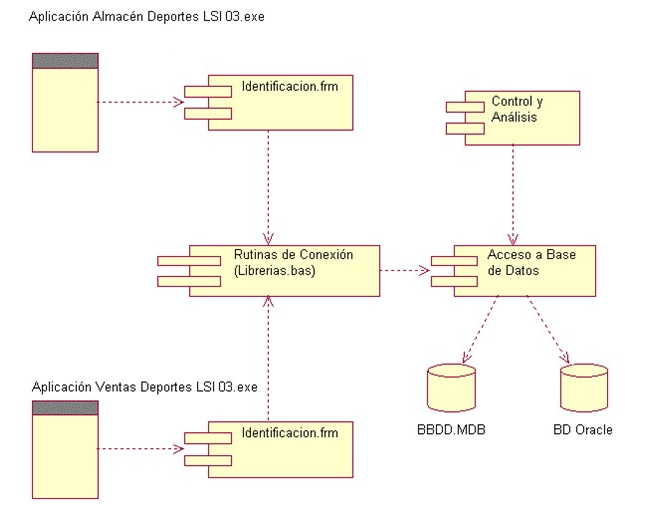
\includegraphics[scale=.4]{Untitled 11.png}}
		\end{figure}
      \end{itemize}
    \item
      Más tipos:

      \begin{itemize}
      \item
        De despliegue: Muestra la distribución de componentes del
        sistema de información con respecto a la partición física.
        Dirigido a diseñadores.
		\begin{figure}[H]
			\ffigbox[\FBwidth]
			{\caption{Diagrama de Despliegue}}
			{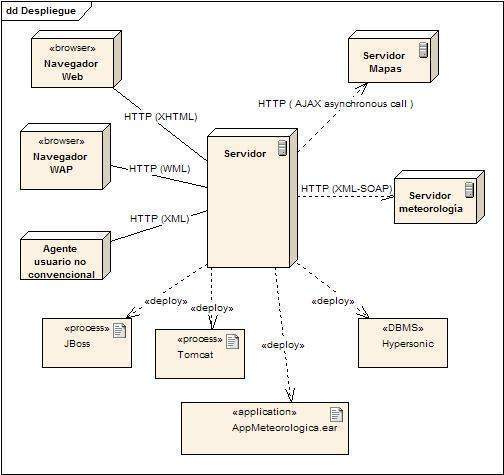
\includegraphics[scale=.4]{Untitled 12.png}}
		\end{figure}
		\pagebreak
      \item
        De actividades: Diagrama de flujo que muestra actividades
        ejecutadas por un sistema.
		\begin{figure}[H]
			\ffigbox[\FBwidth]
			{\caption{Diagrama de Actividades}}
			{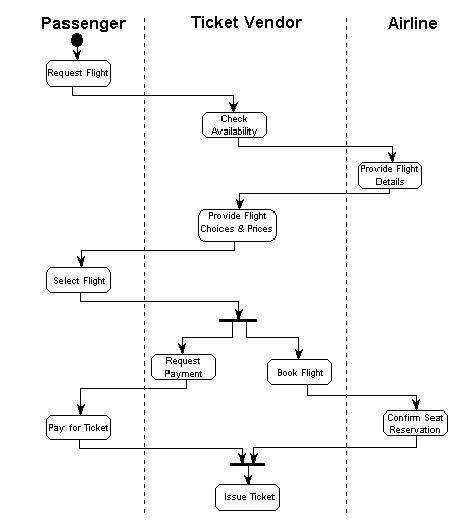
\includegraphics[scale=.5]{Untitled 13.png}}
		\end{figure}
      \item
        De objetos.
      \item
        De secuencia.
      \item
        De colaboración.
      \item
        De tiempo.
      \item
        De interacción.
      \end{itemize}
    \end{itemize}

	Ingeniería directa e inversa
\vspace{-0.5cm}
    \begin{itemize}
    
    \item
      Ingeniería directa: Construir sistemas a partir de lo que los
      modelos especifican.
    \item
      Ingeniería inversa: Representar en modelos sistemas existentes.
    \end{itemize}

	Objetos y clases
	\vspace{-0.5cm}

    \begin{itemize}
    \item
      Objeto: Entidad concreta con identidad, estado y comportamiento.

      \begin{itemize}
      \item
        Un objeto es una instanciación de una clase.
      \item
        Tipos:

        \begin{itemize}
        
        \item
          Objetos físicos.
        \item
          Objetos lógicos.
        \item
          Objetos históricos.
        \end{itemize}
      \item
        Atributos

        Propiedad compartida por los objetos de una clase, cada atributo
        tiene un valor.

        Atributo derivado: Propiedad redundante que puede ser calculada
        a partir de otras.

        visibilidad nombre multiplicidad: Tipo = valorInicial
        \{propiedades\}
      \item
        Operaciones

        Función o transformación que puede aplicarse a los objetos de
        una clase, pueden ser invocadas por otros objetos, o el mismo
        objeto.

        Método: Especificación procedimental de una operación.

        visibilidad nombre (param: Tipo = valDef,\ldots): TipoRet
        \{propiedades\}
      \end{itemize}
    \item
      Clase: Conjunto de entidades abstractas con estructura y
      comportamientos comunes.

      \begin{itemize}
      
      \item
        La clase se usa como plantilla para construir objetos.
      \end{itemize}
    \item
      Análisis: Especificación, vista externa, caja negra.

      \begin{itemize}
      
      \item
        Clases, atributos y operaciones corresponden a conceptos del
        dominio.
      \item
        Es habitual usar una notación simplificada al máximo.
      \end{itemize}
    \item
      Diseño: Implementación, vista interna, caja blanca.

      \begin{itemize}
      
      \item
        Clases, atributos y operaciones corresponden a fragmentos de
        código.
      \item
        Nuevos artefactos y soluciones que dependen del lenguaje y la
        plataforma de implementación.
      \end{itemize}
    \end{itemize}

	Enlace: Conexión entre objetos.

	Asociación: Especificación de un conjunto de enlaces, representan la
    estructura y el comportamiento del sistema.
	\begin{figure}[H]
		\ffigbox[\FBwidth]
		{\caption{Asociación}}
		{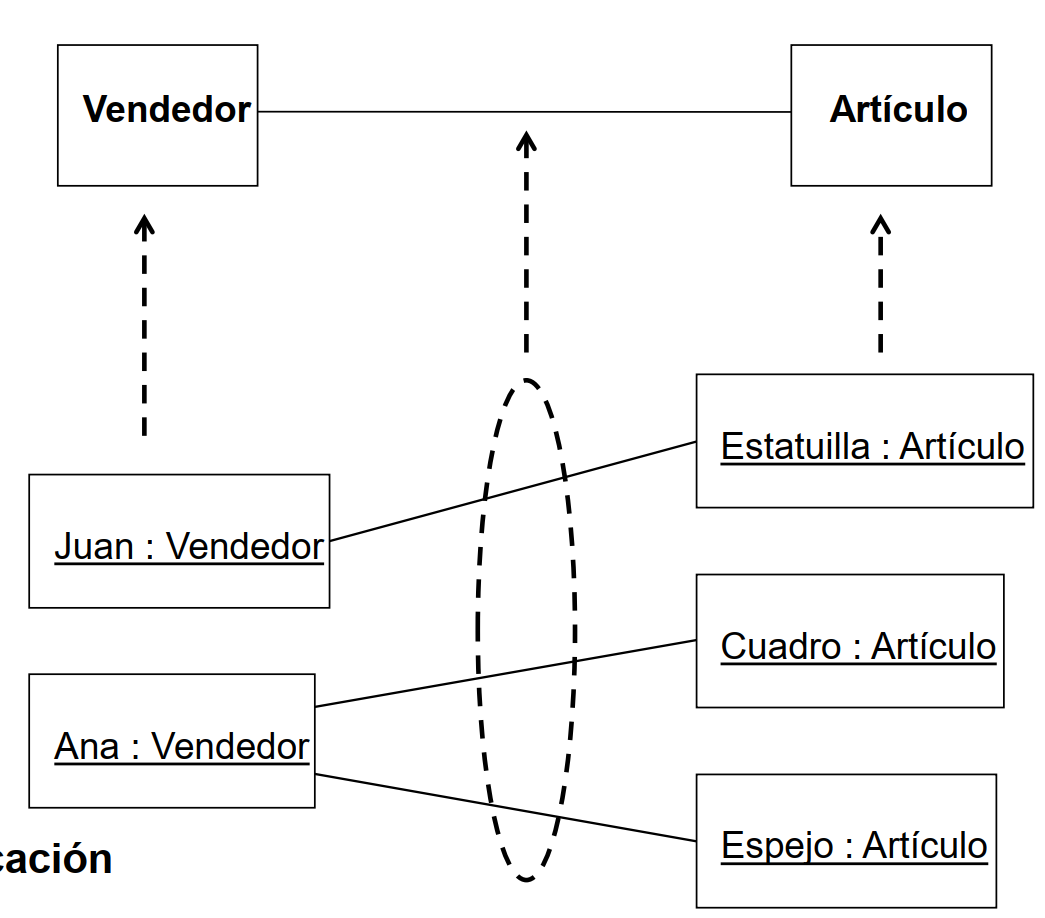
\includegraphics[scale=.2]{Untitled 14.png}}
	\end{figure}
    \begin{itemize}	
    \item
      Nombre de asociación y Dirección del nombre.
	  \begin{figure}[H]
		\ffigbox[\FBwidth]
		{\caption{Nombre y Dirección de asociación}}
		{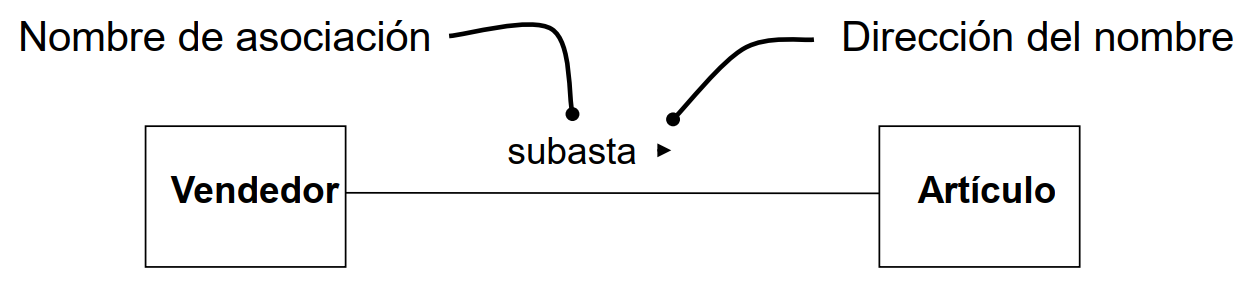
\includegraphics[scale=.3]{Untitled 15.png}}
	\end{figure}
    \item
      Nombres de rol
	  \begin{figure}[H]
		\ffigbox[\FBwidth]
		{\caption{Rol asociación}}
		{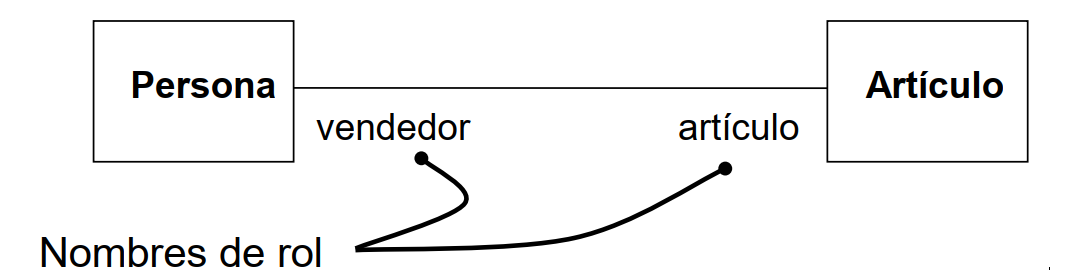
\includegraphics[scale=.3]{Untitled 16.png}}
	\end{figure}
    \item
      Restricciones y notas
	  \begin{figure}[H]
		\ffigbox[\FBwidth]
		{\caption{Restricciones asociación}}
		{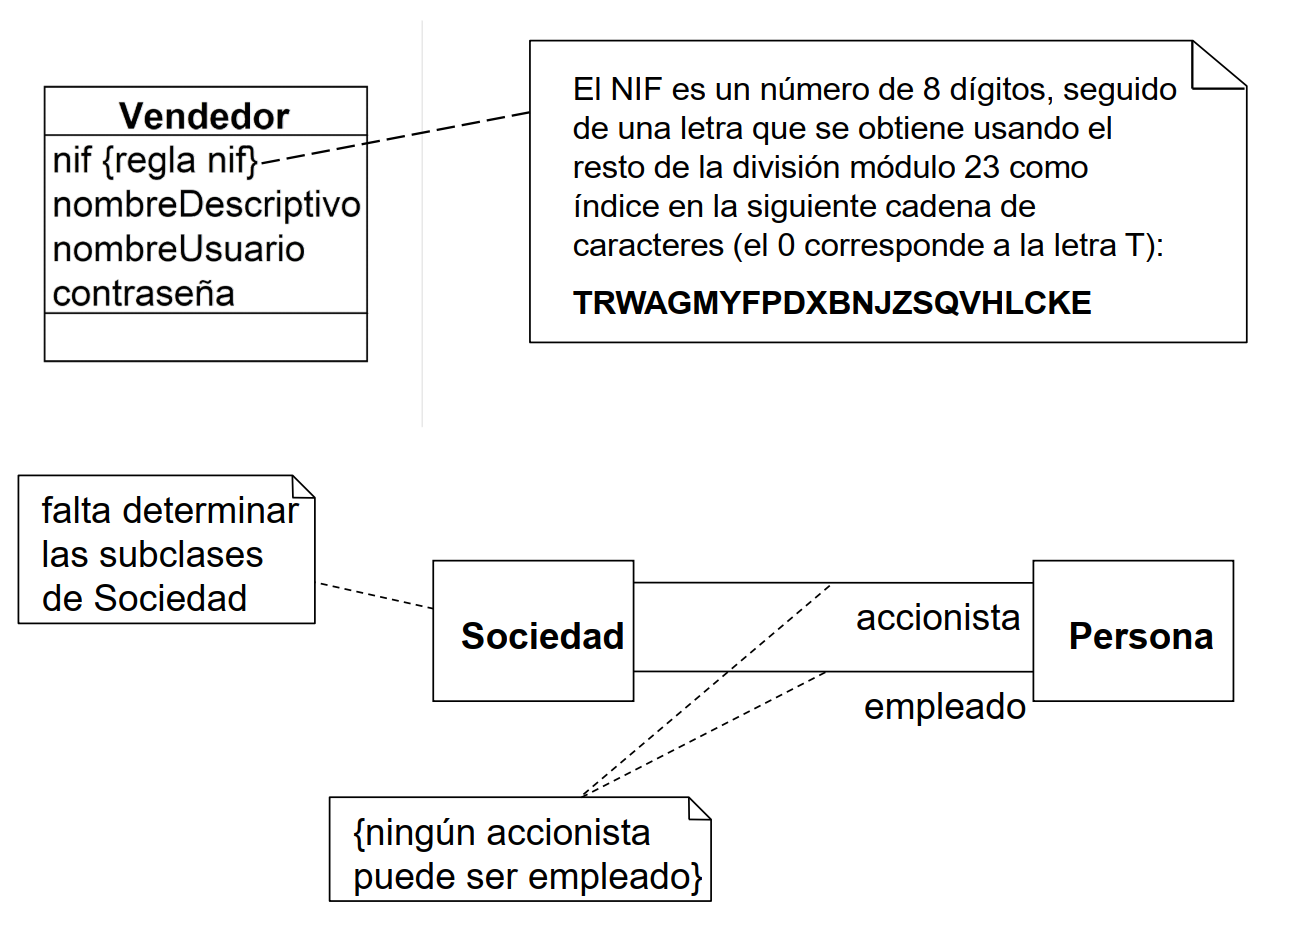
\includegraphics[scale=.3]{Untitled 17.png}}
	\end{figure}
	\pagebreak
    \item
      Multiplicidad de la asociación

      Asociación binaria, la multiplicidad de un extremo de asociación
      específica el número de instancias destino que pueden estar
      enlazadas con una única instancia origen a través de la
      asociación.
	  \begin{figure}[H]
		\ffigbox[\FBwidth]
		{\caption{Multiplicidad de la asociación}}
		{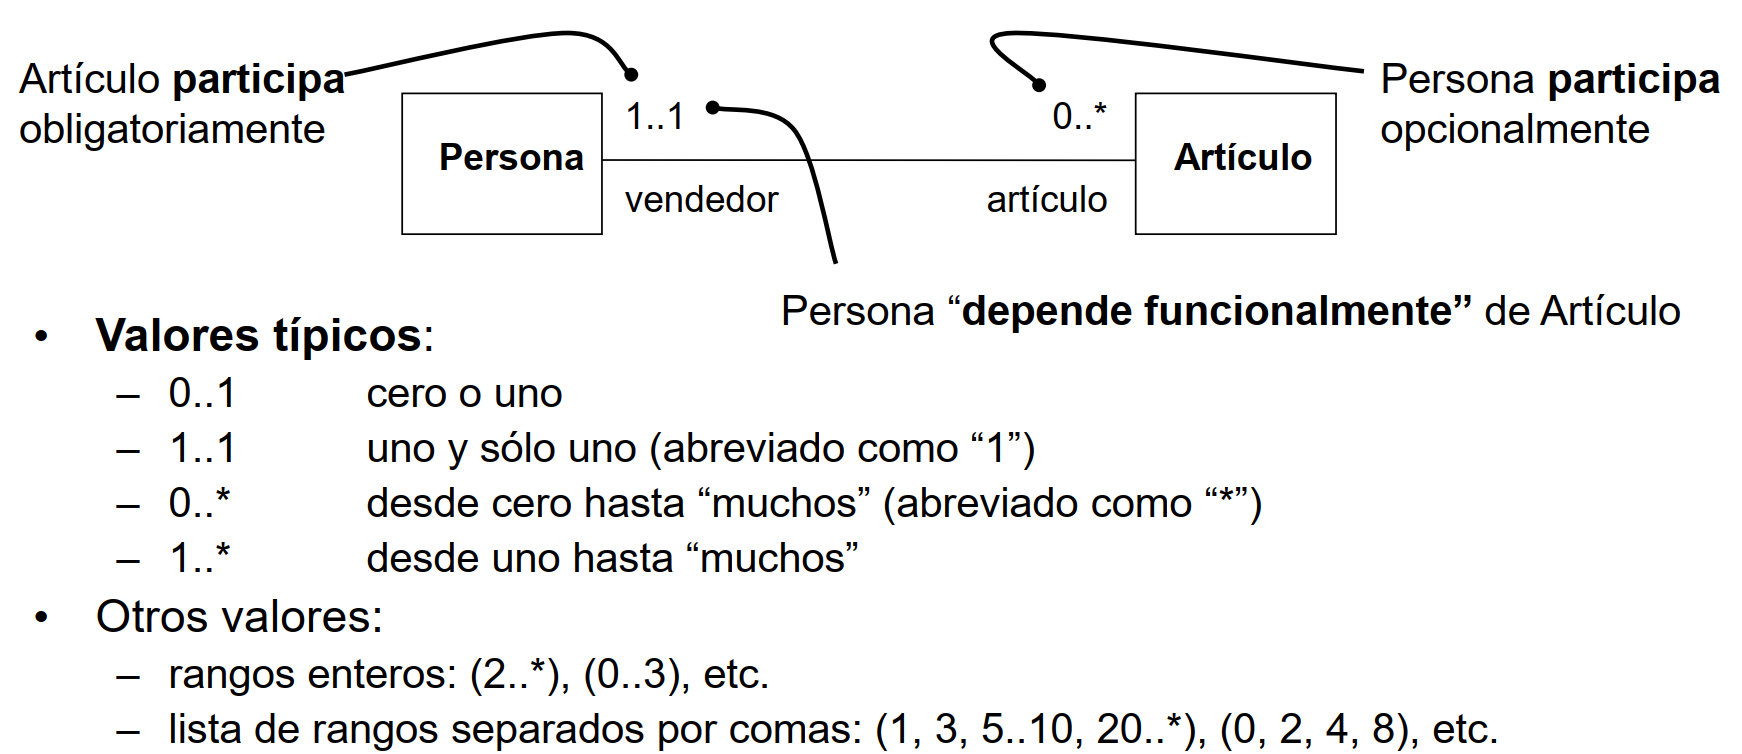
\includegraphics[scale=.22]{Untitled 18.png}}
	\end{figure}
    \item
      Navegabilidad de la asociación.

      Especifica la capacidad que tiene una instancia de la clase origen
      de acceder a las instancias de la clase destino por medio de las
      instancias de la asociación que las conectan.

      Acceder=nombrar, designar o referenciar el objeto para leer o
      modificar atributos, invocar una operación.

      No confundir dirección del nombre con navegabilidad.
	  \begin{figure}[H]
		\ffigbox[\FBwidth]
		{\caption{Navegabilidad de la asociación}}
		{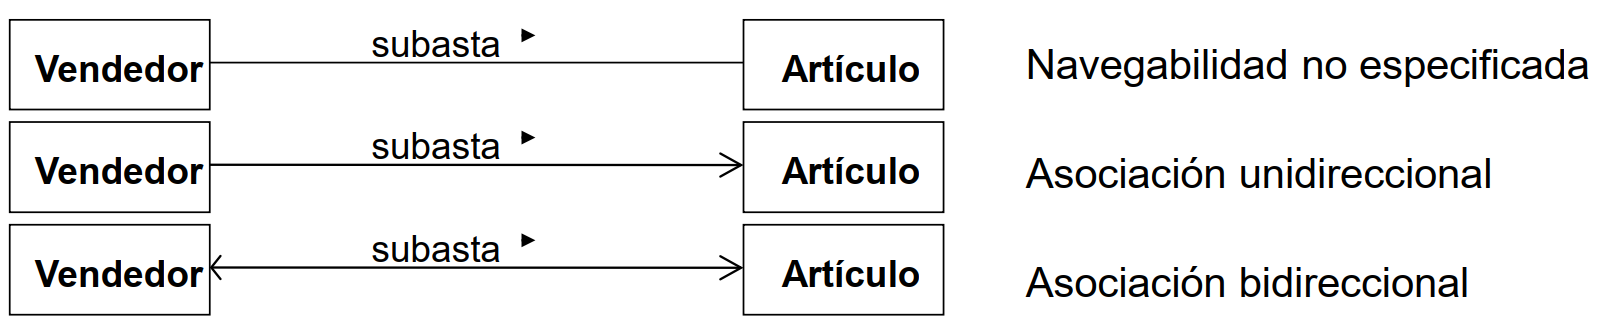
\includegraphics[scale=.23]{Untitled 19.png}}
	\end{figure}
    \item
      Un atributo es equivalente a una asociación unidireccional.
    \item
      Toda asociación tiene doble significado: Aspecto estático y
      aspecto dinámico.

      \begin{itemize}
      
      \item
        Son preferibles los nombres estáticos, reservando los nombres
        dinámicos para nombres de operaciones.
      \item
        Una misma asociación permite la invocación de muchas
        operaciones.
      \end{itemize}
    \item
      Restricciones en asociaciones
	  \begin{figure}[H]
		\ffigbox[\FBwidth]
		{\caption{Restricciones en asociaciones}}
		{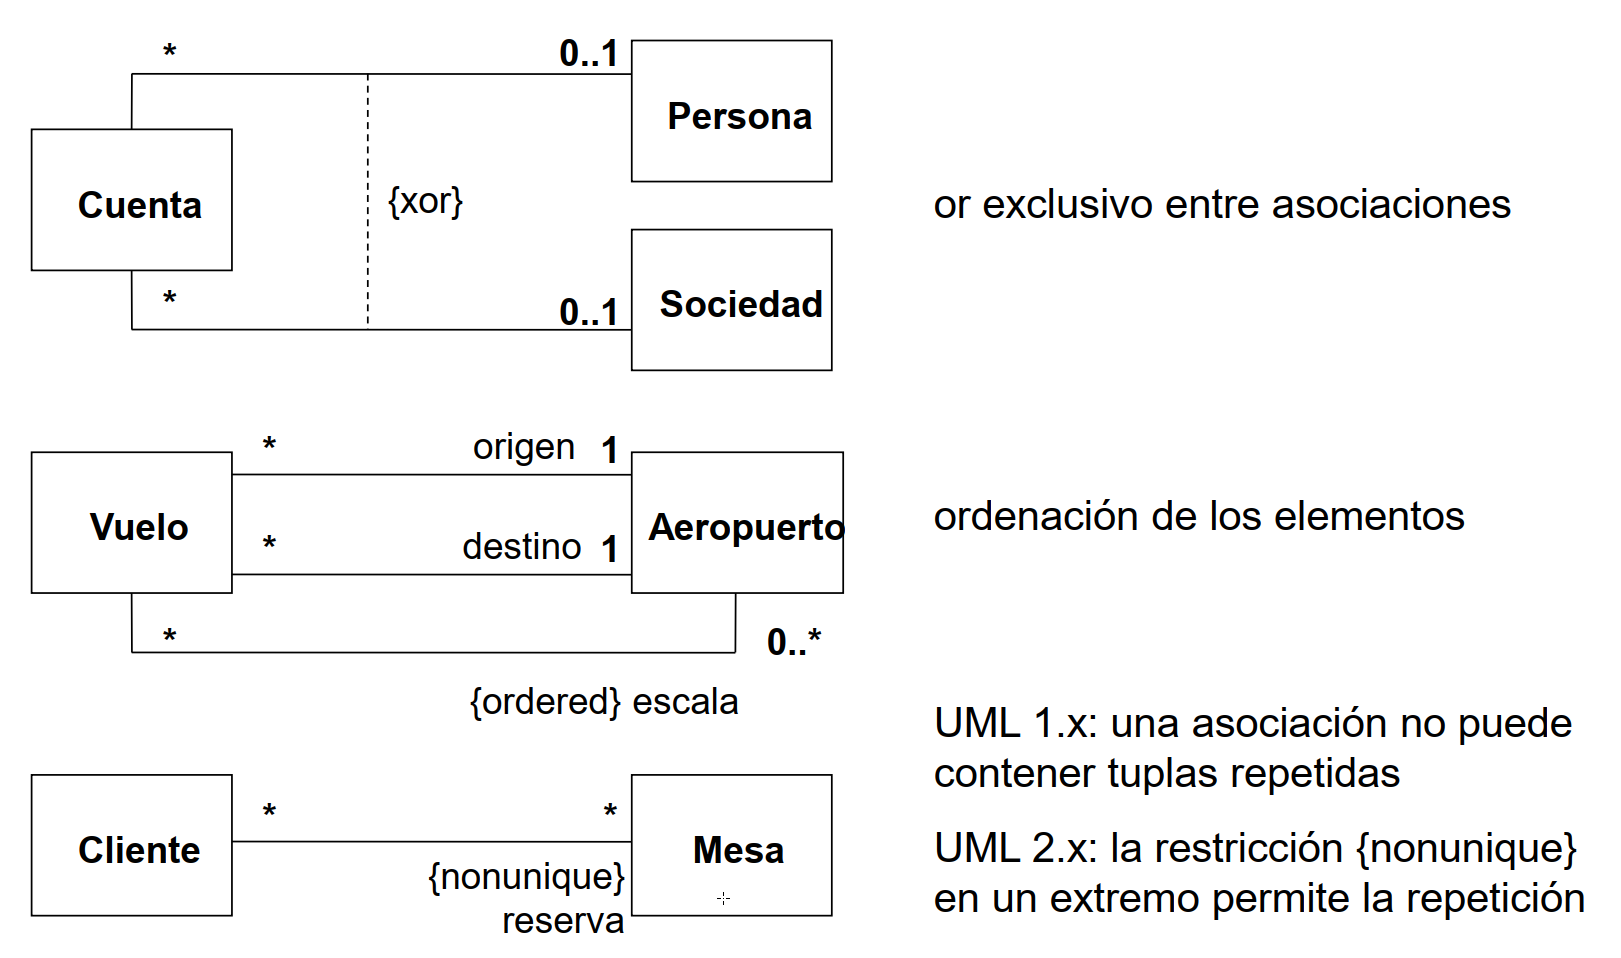
\includegraphics[scale=.23]{Untitled 20.png}}
	\end{figure}
    \item
      Asociaciones actor-sistema y clase-clase

      \begin{itemize}
      
      \item
        Un mismo concepto puede ser modelado a la vez como actor y como
        clase:

        \begin{itemize}
        
        \item
          Actor: representa entidades externas al sistema.
        \item
          Clase: representa entidades modeladas dentro del sistema.
        \end{itemize}
      \end{itemize}
    \end{itemize}

	Asociaciones reflexivas: Es aquella en la que los dos extremos de la
    asociación están unidos a la misma clase.

    \begin{itemize}
    
    \item
      Conectan dos instancias distintas de la misma clase o incluso una
      instancia consigo mismo.
    \item
      Los nombres de rol son obligatorios.
    \item
      No es simétrica.
	  \begin{figure}[H]
		\ffigbox[\FBwidth]
		{\caption{Asociación reflexiva}}
		{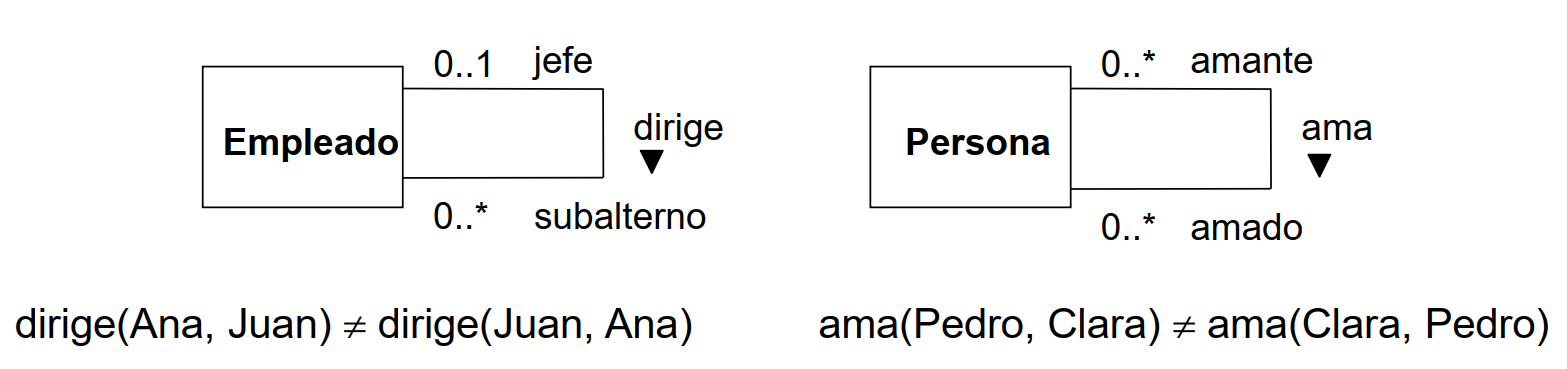
\includegraphics[scale=.26]{Untitled 21.png}}
	\end{figure}
    \end{itemize}
\pagebreak
	Asociación n-aria

    \begin{itemize}
    \item
      Asociación entre N clases, los enlaces conectan N instancias.

      \begin{itemize}
      
      \item
        No permite: dirección del nombre, agregación.
      \item
        Si permite: navegabilidad, clase asociación.
      \end{itemize}
    \item
      Multiplicidad engañosa.
	  \begin{figure}[H]
		\ffigbox[\FBwidth]
		{\caption{Asociación n-aria}}
		{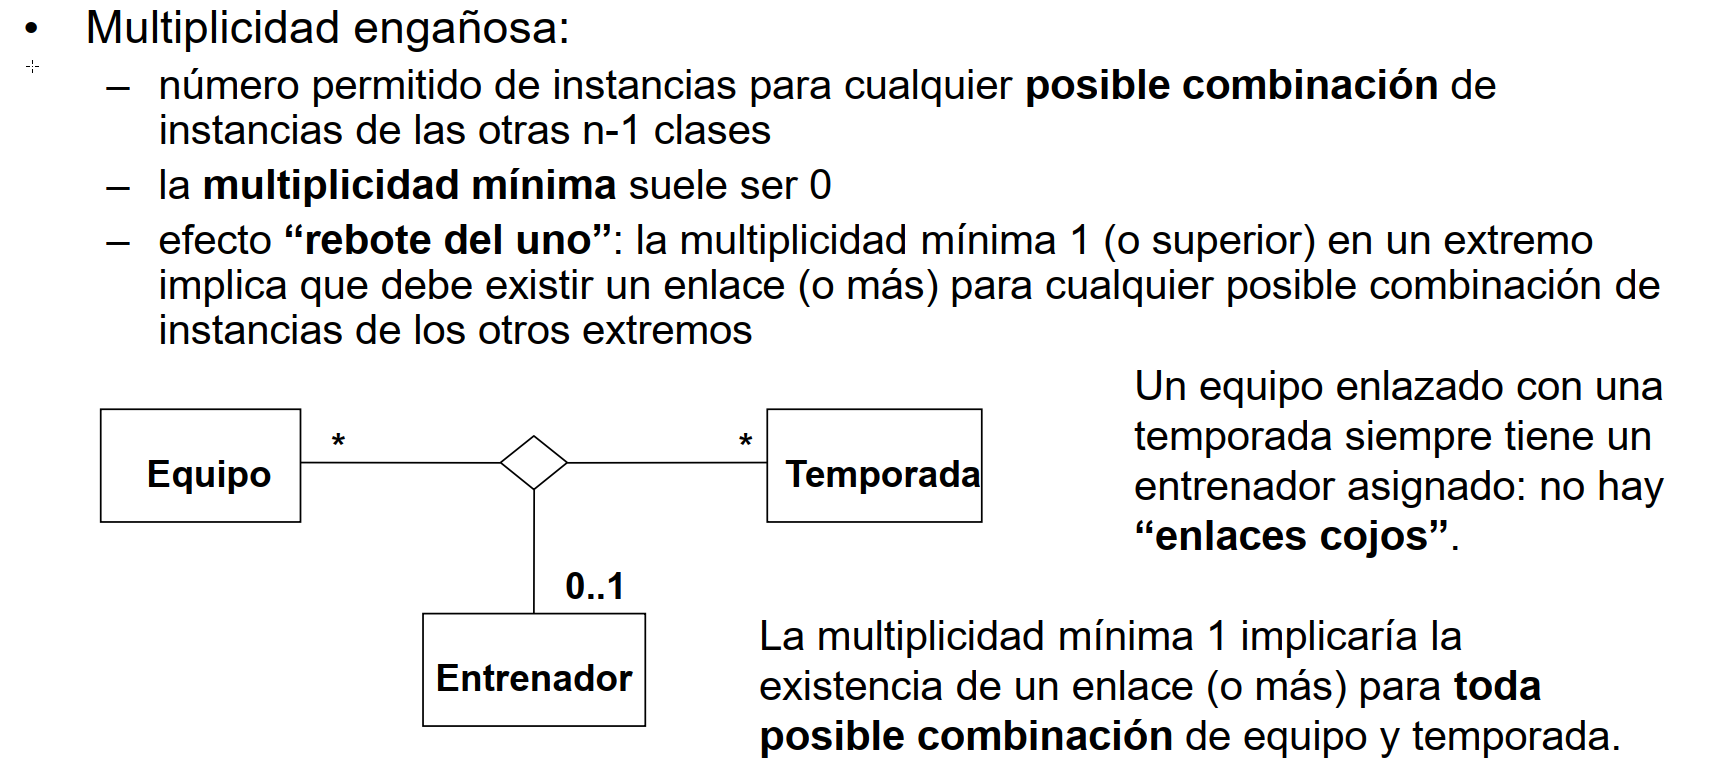
\includegraphics[scale=.2]{Untitled 22.png}}
	\end{figure}
    \item
      Se puede sustituir la asociación n-aria por una clase simple,
      cuyas instancias representan enlaces.
    \item
      Se pierden las multiplicidades originales.
    \item
      Clase-asociación

      \begin{itemize}
      \item
        Tiene todas las propiedades de una clase y de una asociación:

        \begin{itemize}
        
        \item
          Atributos, operaciones y asociaciones con otras clases.
        \item
          Conexión entre clases que especifica enlaces entre ellas.
        \item
          Multiplicidad, navegabilidad, agregación\ldots{}
        \end{itemize}
      \item
        Tiene nombre único.
		\begin{figure}[H]
			\ffigbox[\FBwidth]
			{\caption{Clase-asociación}}
			{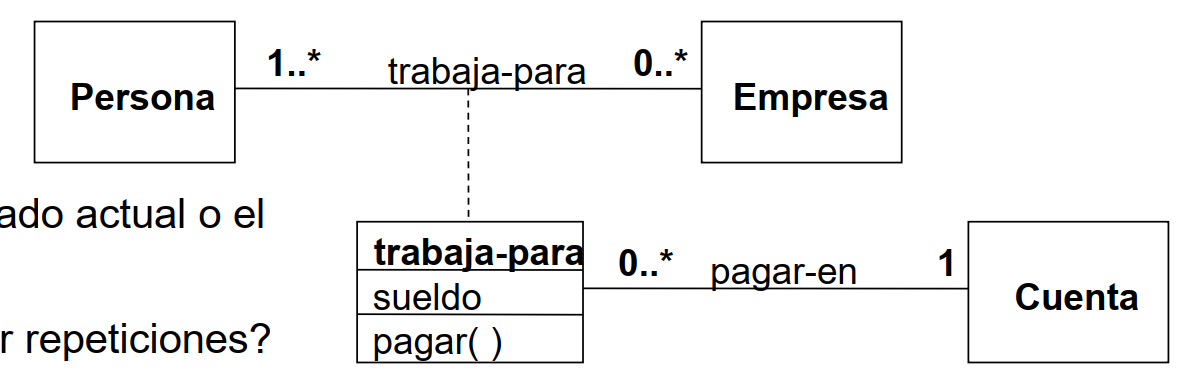
\includegraphics[scale=.25]{Untitled 23.png}}
		\end{figure}
      \item
        Se puede transformar en clase intermedia, cuyas instancias
        representan enlaces.
      \item
        Las multiplicidades originales se cruzan.
		\begin{figure}[H]
			\ffigbox[\FBwidth]
			{\caption{Multiplicidad Clase-asociación}}
			{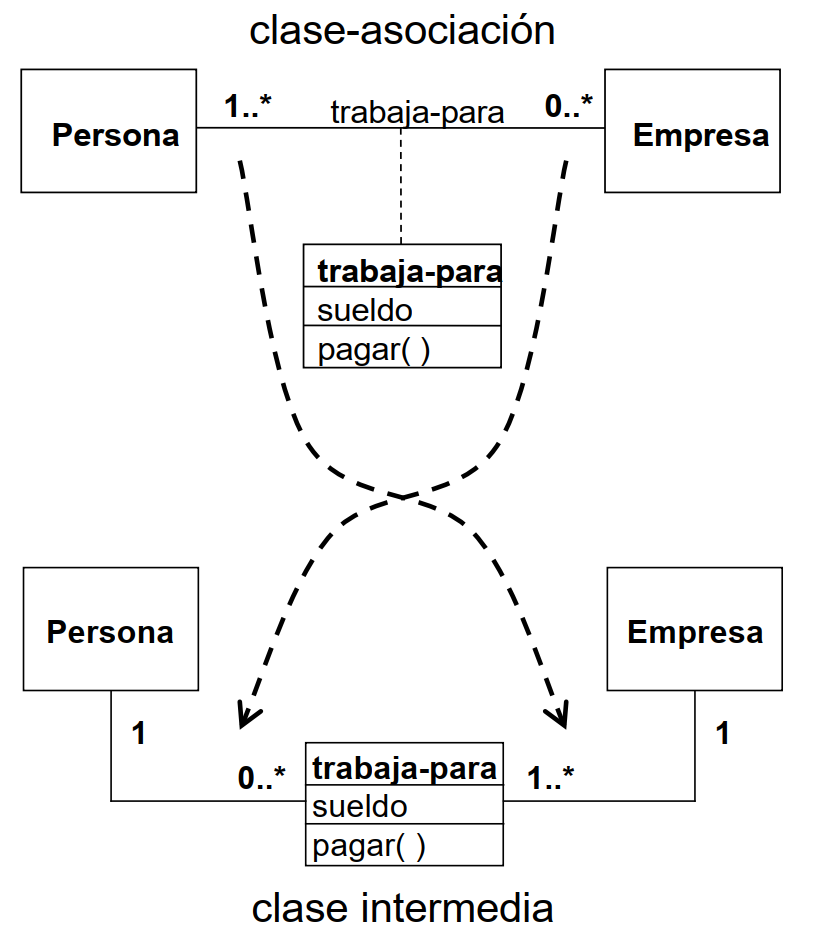
\includegraphics[scale=.25]{Untitled 24.png}}
		\end{figure}
      \end{itemize}
    \end{itemize}

	Generalización y clasificación

    \begin{itemize}
    
    \item
      Principio de sustitución:

      \begin{itemize}
      
      \item
        Extensión: todos los objetos de la subclase son también de la
        superclase.
      \item
        Intensión: la definición de la superclase es aplicable a la
        subclase.
      \end{itemize}
    \item
      Generalización: clase-clase.
    \item
      Clasificación: objeto-clase.
    \end{itemize}

	Generalización y especialización

    \begin{itemize}
    
    \item
      Generalizar es identificar las propiedades comunes (atributos,
      asociaciones, operaciones) de varias clases y representarlas en
      una clase más general denominada superclase.
    \item
      Especializar es capturar las propiedades específicas de un conjunto
      de objetos dentro de una clase dada, que aún no han sido
      distinguidas en ella, y representarlas en una nueva clase
      denominada subclase.
	  \pagebreak
    \item
      Es una relación pura entre clases:

      \begin{itemize}
      
      \item
        No tiene instancias, ni multiplicidad.
      \item
        La subclase hereda todas las propiedades de la superclase.
      \item
        Las propiedades heredadas de la superclase no se representan en
        la subclase (a menos que sean operaciones redefinidas).
      \item
        Toda generalización induce una dependencia subclase Æ superclase
      \end{itemize}
    \end{itemize}

	Generalización múltiple vs. Clasificación múltiple
	\begin{figure}[H]
		\ffigbox[\FBwidth]
		{\caption{Generalización múltiple vs. Clasificación múltiple}}
		{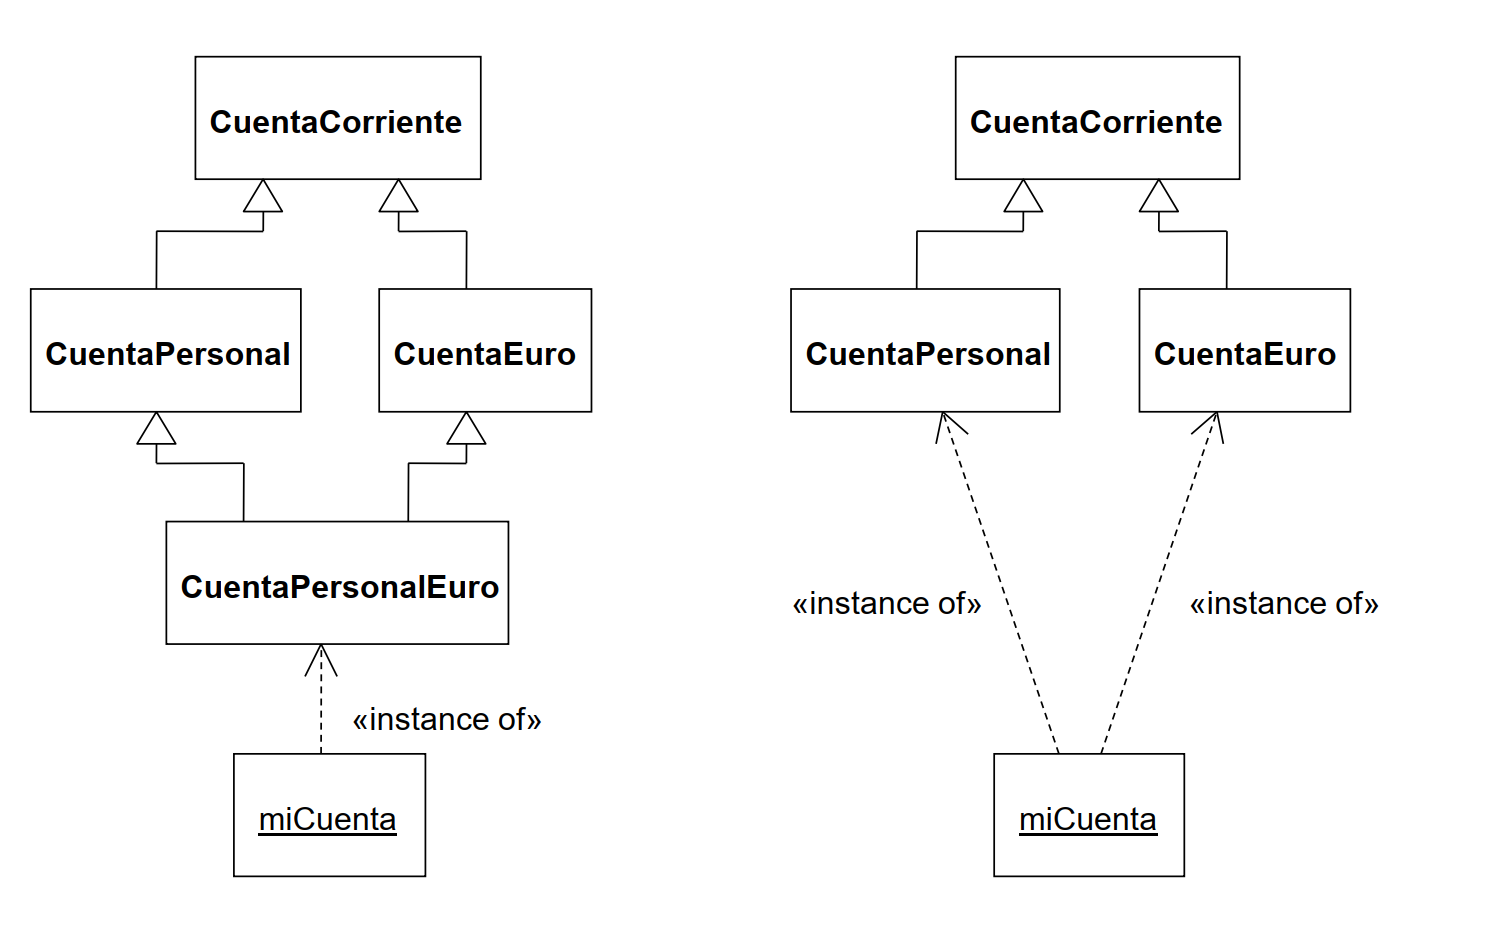
\includegraphics[scale=.2]{Untitled 25.png}}
	\end{figure}

	Subclase vs. Atributo

    \begin{itemize}
    
    \item
      Atributo: Para propiedades cambiantes o rangos de valores muy
      altos.
    \item
      Subclase: Para propiedades fijas con valores enumerados,
      especificación.
    \item
      Permite modelar un cambio de propiedad como una reclasificación
      del objeto.
    \end{itemize}

	Agregación    \vspace{-0.5cm}

	\begin{figure}[H]
		\ffigbox[\FBwidth]
		{\caption{Agregación}}
		{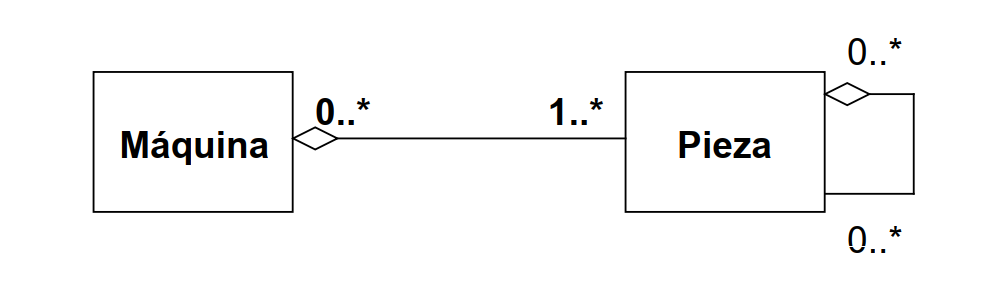
\includegraphics[scale=.2]{Untitled 26.png}}
	\end{figure}
    \begin{itemize}
    \vspace{-0.5cm}
    \item
      Es un tipo especial de asociación que representa una relación
      todo-parte, transitiva y asimétrica.

      \begin{itemize}
      
      \item
        impone ninguna restricción especial sobre la multiplicidad
      \end{itemize}
    \end{itemize}

	Composición
	\begin{figure}[H]
		\ffigbox[\FBwidth]
		{\caption{Composición}}
		{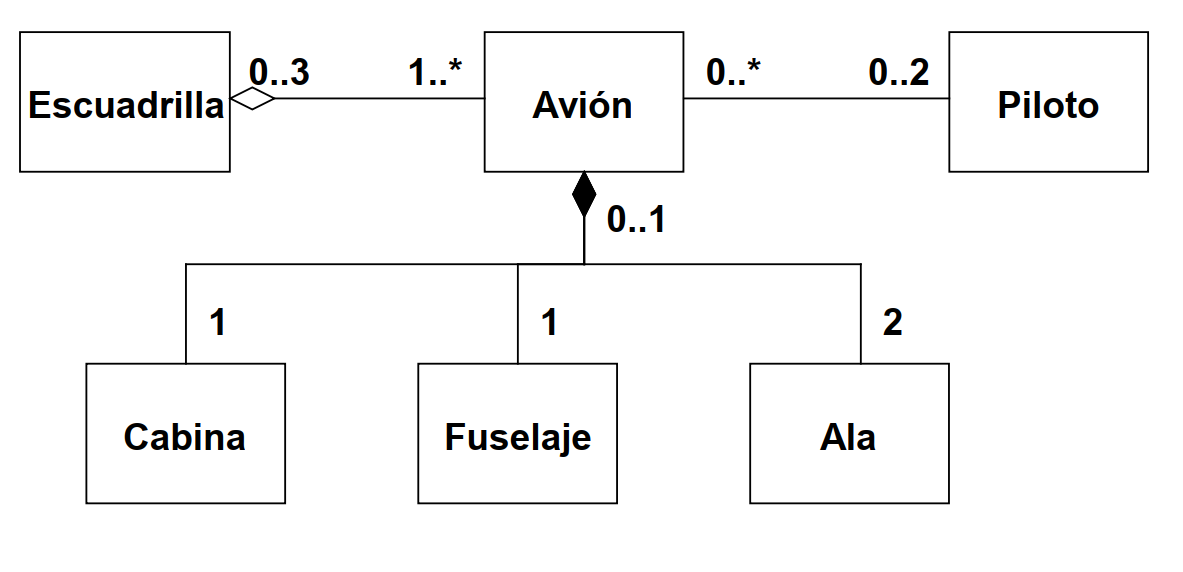
\includegraphics[scale=.2]{Untitled 27.png}}
	\end{figure}
    \begin{itemize}
    
    \item
      Es un tipo especial de agregación no compartida

      \begin{itemize}
      
      \item
        la multiplicidad solo puede ser 0..1 o 1..1
      \item
        el todo es responsable de la existencia y almacenamiento de las
        partes
      \item
        propagación de las operaciones de copiado y borrado
      \end{itemize}
    \end{itemize}

	Diagrama de clases: Captura y especifica y vocabulario del sistema:

    \begin{itemize}
    
    \item
      elementos: clases, atributos, operaciones\ldots{}
    \item
      relaciones: asociaciones, generalizaciones, composición,
      agregación\ldots{}
    \item
      estructura del sistema, fundamento de su comportamiento.
	  \begin{figure}[H]
		\ffigbox[\FBwidth]
		{\caption{Diagrama de clases}}
		{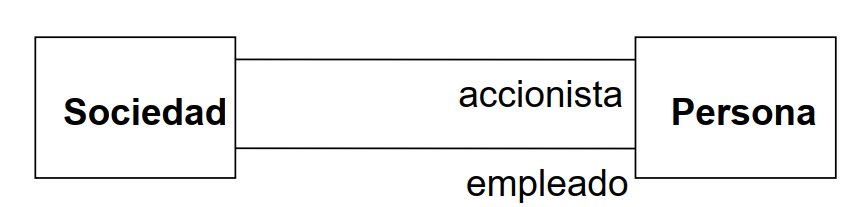
\includegraphics[scale=.25]{Untitled 28.png}}
	\end{figure}
    \end{itemize}

    Sugerencias para mejorar la comunicación:

    \begin{itemize}
    
    \item
      nombres adecuados: clases, atributos, operaciones, asociaciones,
      roles
    \item
      distribución espacial de los elementos
    \item
      evitar cruces de líneas
    \item
      distinto nivel de detalle según el propósito y nivel de
      abstracción
    \end{itemize}
\pagebreak
	Diagrama de objetos

    \begin{itemize}
    
    \item
      ilustra la estructura del sistema mediante situaciones
      particulares.
    \item
      Muestra objetos, valores de atributos y enlaces.
    \end{itemize}
	\begin{figure}[H]
		\ffigbox[\FBwidth]
		{\caption{Diagrama de Objetos}}
		{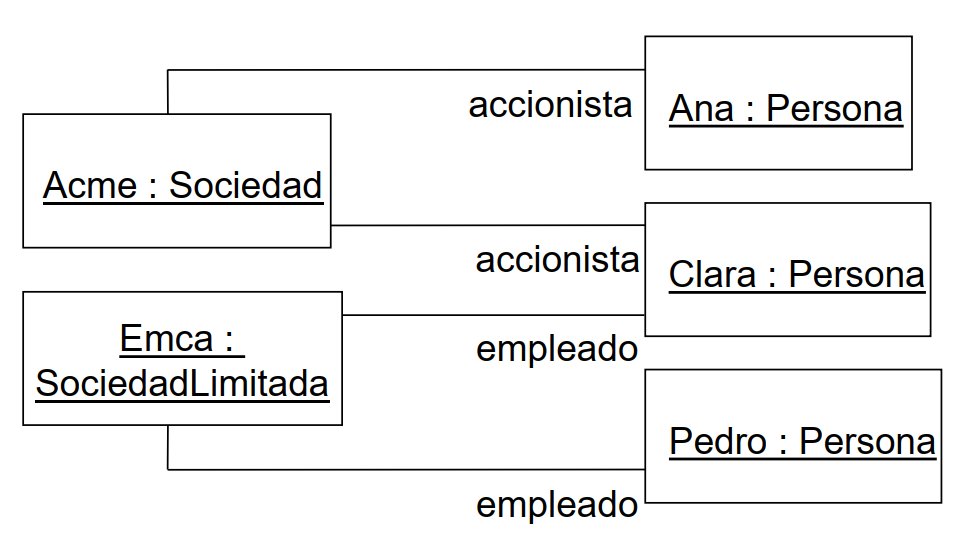
\includegraphics[scale=.3]{Untitled 29.png}}
	\end{figure}
  
\chapter{TEMA 3 - Arquitectura}


La definición que mejor lo transmite:

\begin{itemize}
\item
	La arquitectura del software es la organización fundamental de un
	sistema encarnada en sus componentes, las relaciones entre ellos y
	con el entorno, y los principios que orientan su diseño y
	evolución.
\end{itemize}

Es como vamos a organizar los componentes/bloques del sistema, la
relación entre ellos y también su relación con el entorno.

Modelo 4+1: Las vistas son como dimensiones, nos dan una
aproximación distinta.

\begin{itemize}
    \item Vista lógica (conceptual).
		\begin{itemize}
			
			\item
				Diagramas de clases, modelado, y asociaciones, relaciones entre
				clases.
			\item
				El propósito es especificar la arquitectura de información del
				sistema que se desea construir, mediante un conjunto de
				diagramas de clases adecuadamente explicados.
			\item
				El modelo de información, o modelo conceptual, debe estar
				justificado a partir de los requisitos. No tiene sentido que en
				él aparezcan clases, atributos, operaciones y otros elementos
				que no hayan aparecido anteriormente en los requisitos.
				Igualmente, no tiene sentido que en los requisitos se mencionen
				conceptos importantes que no aparezcan reflejados de ninguna
				manera en el modelo conceptual.
			\item
				El vocabulario del modelo conceptual define todos los términos
				significativos y específicos del problema que parecen en los
				requisitos. Es un puente importante que vincula los requisitos
				con el modelo conceptual.
		\end{itemize}
    \item Vista de desarrollo (implementación).
    	\begin{itemize}
      
			\item
				Organización del software.
			\item
				Habla de los bloques/componentes del sistema y sus relaciones.
			\item
				Interesados: Programadores.
			\item
				Diagramas de componentes y relaciones de uso.
			\item
				Define la descomposición del sistema en subsistemas y
				componentes, y se especifican las dependencias entre los
				distintos componentes que hayan resultado de la descomposición
			\pagebreak
			\item
				Los componentes se refieren a:
				\begin{itemize}
					\item
					Elementos estático y estructurales del sistema que representa
					una funcionalidad concreta o un conjunto de ellas utilizados
					en la implementación: funciones, librerías, etc.
					\item
					Conjunto de datos usados en la implementación: ficheros, bases
					de datos, etc.
				\end{itemize}
			\item
				La arquitectura de desarrollo se representa a través de los
				diagramas de componentes.
			\item
				Componentes vs. Clases
				\begin{itemize}
					\item
					Se parecen a las clases en que tienen nombres, realizan
					interfaces, pueden participar en relaciones,
					\item
					Pero se diferencian en que las clases son abstracciones
					lógicas (se instancian como objetos) y los componentes son
					fragmentos físicos.
				\end{itemize}
			\item
				Componentes e interfaces
				\begin{itemize}
					\item
					Definen su comportamiento en base a interfaces requeridas y
					ofertadas.
					\item
					Unos componentes implementan las interfaces y otros acceden a
					los servicios proporcionados por esas interfaces.
				\end{itemize}
			\item
				Estas relaciones se pueden mostrar con dos tipos de notación:
				icónica o expandida.
				\begin{figure}[H]
					\ffigbox[\FBwidth]
					{\caption{Componentes e interfaces}}
					{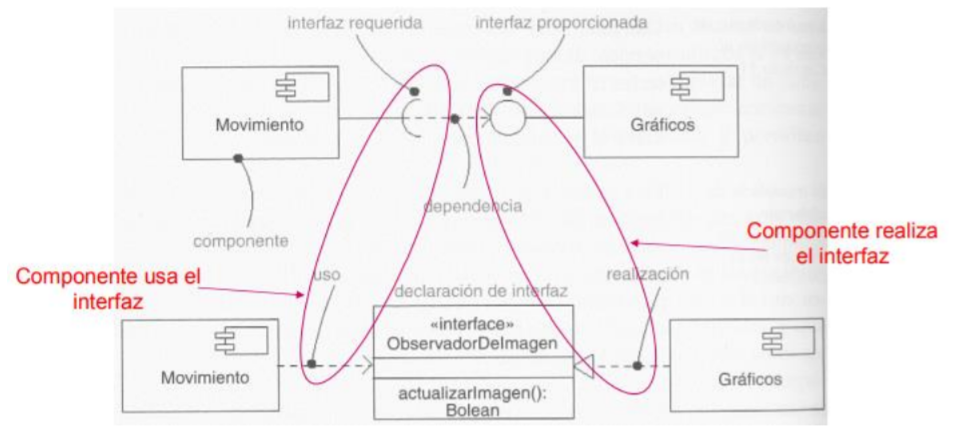
\includegraphics[scale=.3]{Untitled 30.png}}
				\end{figure}
		\end{itemize}
    \item
      Vista de proceso (ejecución). No lo veremos.
    \item
      Vista física (despliegue). No lo veremos.
    \item
      Vista de casos de uso. La hemos visto, es del modelado conceptual.
\end{itemize}
\pagebreak
Diseñar una arquitectura: pasos

\begin{itemize}
	\item Buscar los patrones más apropiados que den el soporte requerido
		para alcanzar los atributos de calidad deseados
		\begin{itemize}
			\item Basarse en Arquitecturas de Referencia reconocidas por tanto por
			la academia como por la industria
 			\begin{itemize}
		
				\item
					Implementaciones conocidas, de amplia difusión y uso
				\item
					Buena documentación
			\end{itemize}
			\item Reconocer el tamaño de la aplicación objetivo
			\begin{itemize}
				\item
					Aplicaciones pequeñas: Pocos patrones requeridos
				\item
					Aplicaciones grandes: Mezcla de varios patrones
			\end{itemize}
			\item Debe justificarse teniendo en cuenta:
			\begin{itemize}
				\item
					Los criterios: simplicidad, extensibilidad, modificabilidad,
					eficiencia.
				\item
					Los requisitos no funcionales.
				\item
					Otros que se consideren relevantes: habilidades técnicas,
					costes.
			\end{itemize}
		\end{itemize}
	\item Identificación de módulos: subsistemas y componentes
		\begin{itemize}
			\item
			La clasificación de requisitos por áreas temáticas puede también
			proporcionar pistas importantes para esta descomposición.
			\item
			Asignación de componentes
			\begin{itemize}
				\item
					Identificar los componentes principales
				\item
					Identificar como los componentes se ajustan a los patrones
				\item
					Identificar dependencias entre ellos
				\item
					Identificar las interfaces y los servicios que cada componente
					soporta
			\end{itemize}
		\end{itemize}
\end{itemize}

Como lograr una buena descomposición modular:

\begin{itemize}
	\item Buen diseño: Bajo acoplamiento y Alta cohesión.
	\item Acoplamiento: El número de líneas que hay entre dos subsistemas
		distintos.
	\item Cohesión: La relación entre los componentes de un subsistema. Si
		hay relaciones, está muy cohesionado.
	\pagebreak
	\item Ejemplo
	\begin{figure}[H]
		\ffigbox[\FBwidth]
		{\caption{Descomposición modular}}
		{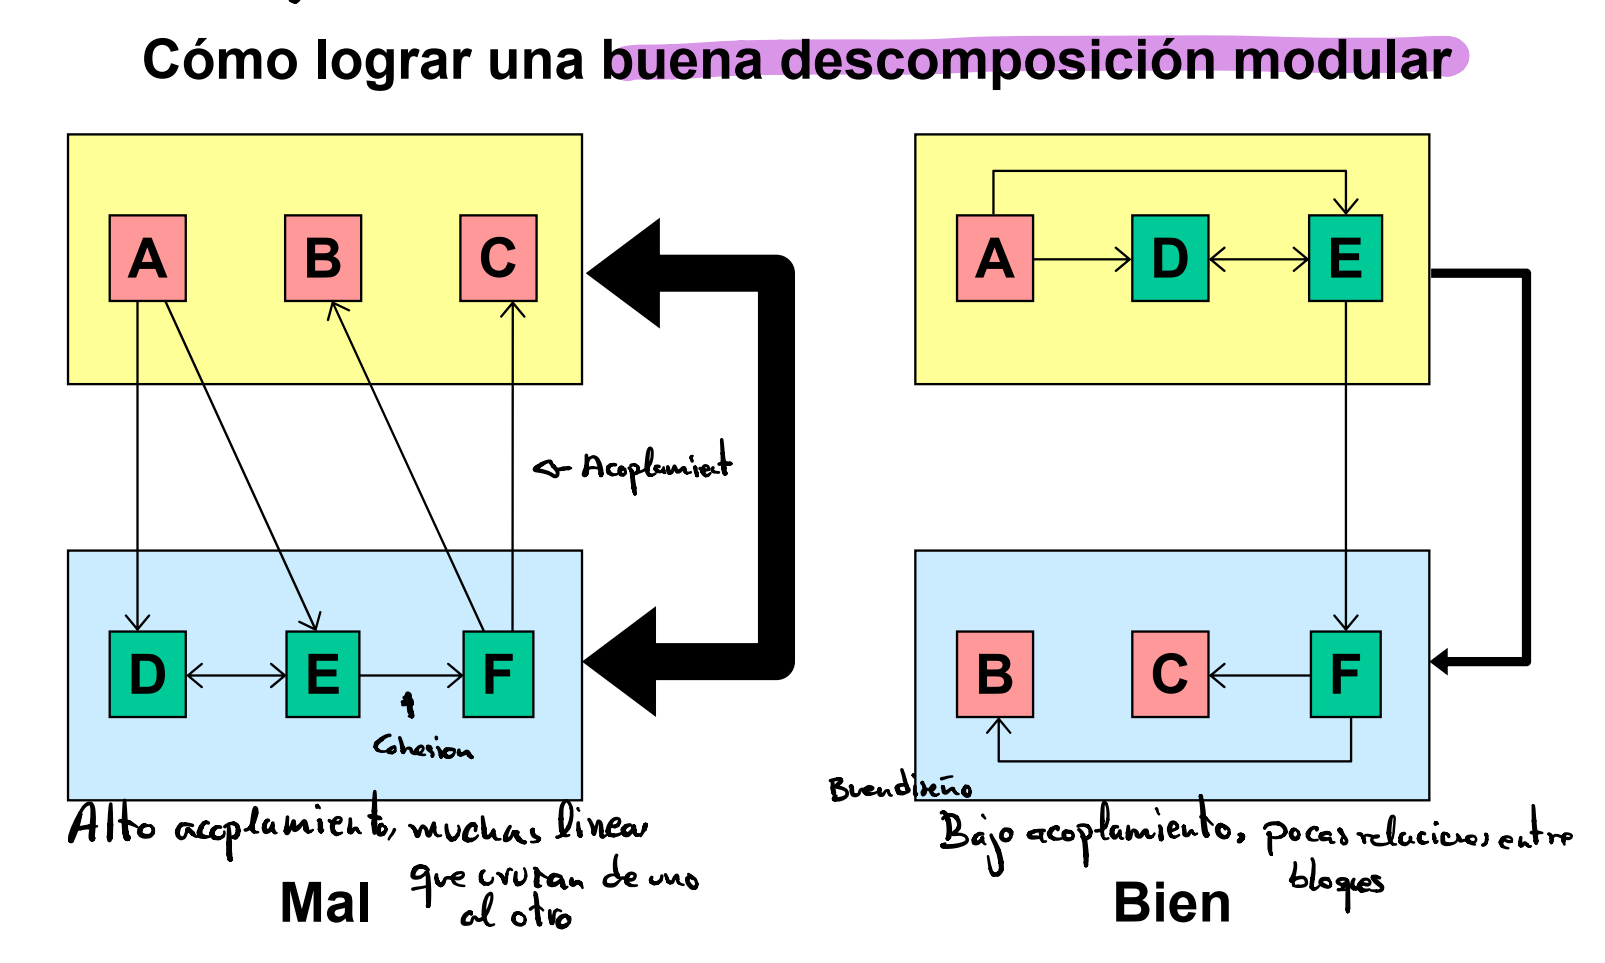
\includegraphics[scale=.25]{Untitled 31.png}}
	\end{figure}

\end{itemize}

Criterios para la selección de una arquitectura:

\begin{itemize}
	\item Criterios clásicos:
		\begin{itemize}
			\item Extensibilidad: Que puede evolucionar, se facilita la adición de
			nuevas características.
				\begin{itemize}
					\item Hace más complejo el diseño.
					\item Mayor grado de abstracción.
					\item Distinguir entre opcionales y deseables es muy útil.
				\end{itemize}
			\item Modificabilidad: facilitar el cambio de requisitos.
			\item Simplicidad: hacer fácil de entender, hacer fácil de
			implementar.
			\item Eficiencia: Lograr alta velocidad o pequeño tamaño.
		\end{itemize}
	\item Otros criterios: Reúso, Escalabilidad, Coste, Requisitos no
		funcionales\ldots{}
\end{itemize}
\pagebreak
Componentes:
\begin{itemize} 
    \item Definición:
		\begin{itemize}
			\item Partes modulares de un sistema (pieza ejecutable de software)
			\item Independientes entre sí.
			\item Autocontenidos, encapsulan las estructuras que contienen.
			\item Los elementos encapsulados en un componente se comunican con
				otros elementos de otros componentes mediante interfaces.
			\item Interfaces: En un diagrama de componentes, documentan las
				relaciones y dependencias en una arquitectura de software.
			\item Modelan los sistemas de cara a la implementación.
      	\end{itemize}
    \item Componentes: En UML es una definición muy amplia, se utiliza para
      denominar varias partes del sistema, como bases de datos,
      paquetes, archivos y bibliotecas. También componentes
      especializados relacionados con los ámbitos y procesos.
\end{itemize}

Se usan diagramas de componentes por:
\begin{itemize} 
    \item Visión general del sistema y documenta la organización de los
      componentes del sistema y sus relaciones y dependencias mutuas.
    \item Visión orientada a la ejecución, es decir, dan al desarrollador
      información.
    \item Especificación de arquitecturas de software y al división de
      sistemas en subsistemas.
    \item Facilitan la gestión del desarrollo de programas.
    \item Reutilización: Permiten visualizar de forma clara que bloques
      modulares se pueden utilizar varias veces en varios puntos de una
      arquitectura.
\end{itemize}

Los componentes se representan con <<component>> y la
cajita con dos rayas.
\begin{figure}[H]
	\ffigbox[\FBwidth]
	{\caption{<<component>>}}
	{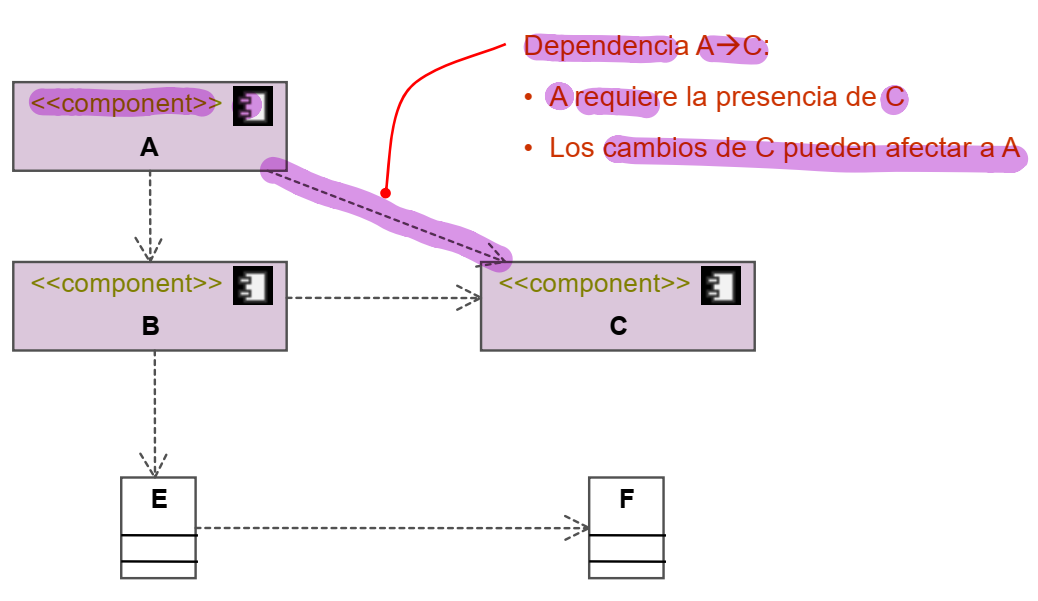
\includegraphics[scale=.3]{Untitled 32.png}}
\end{figure}

Las relaciones son de dependencia, apunta del que depende. De tal
manera que los cambios del destino afectan al origen de la relación.
\begin{figure}[H]
	\ffigbox[\FBwidth]
	{\caption{Ej. Relación de depndendencia}}
	{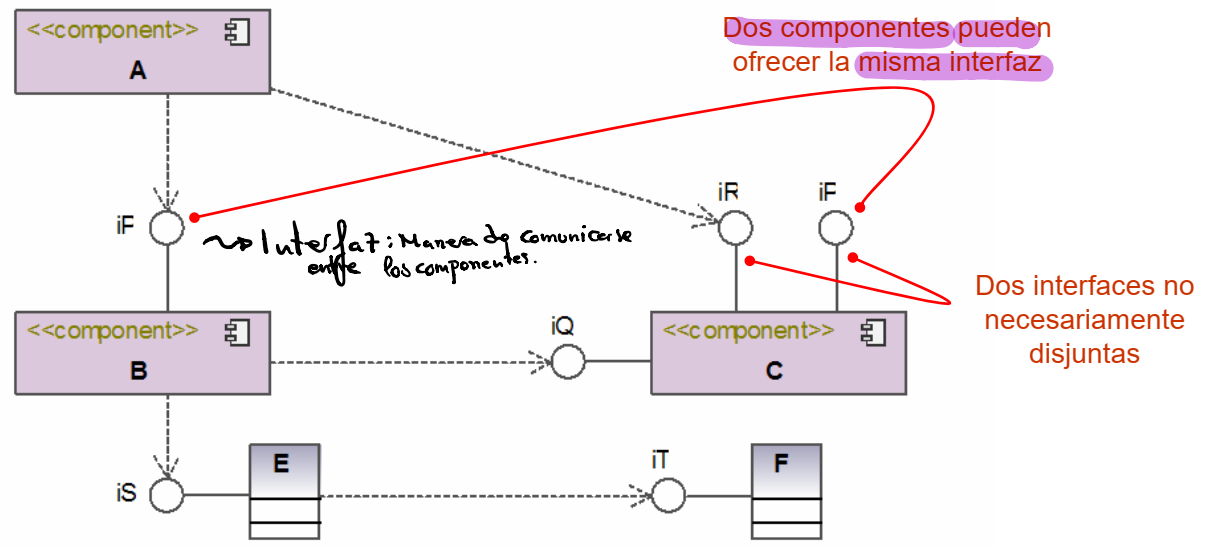
\includegraphics[scale=.3]{Untitled 33.png}}
\end{figure}
\pagebreak
Representación de elementos de diagramas de componentes.
\begin{figure}[H]
	\ffigbox[\FBwidth]
	{\caption{Resumen elementos diagrama dec componentes}}
	{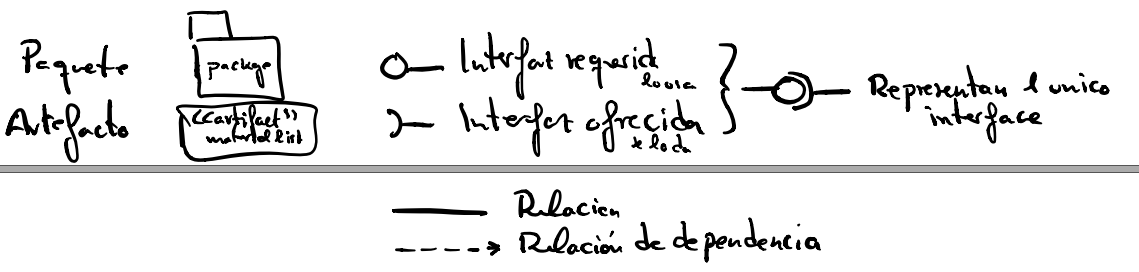
\includegraphics[scale=.3]{Untitled 34.png}}
\end{figure}
\begin{itemize}
	\item LO DE REQUERIDA Y OFRECER ES AL REVÉS.
	\item Usaremos: Componente, Paquete (subsistema), Interfaz ofrecida,
	Interfaz requerida y Relación.
\end{itemize}

\begin{figure}[H]
	\ffigbox[\FBwidth]
	{\caption{Elementos diagrama dec componentes}}
	{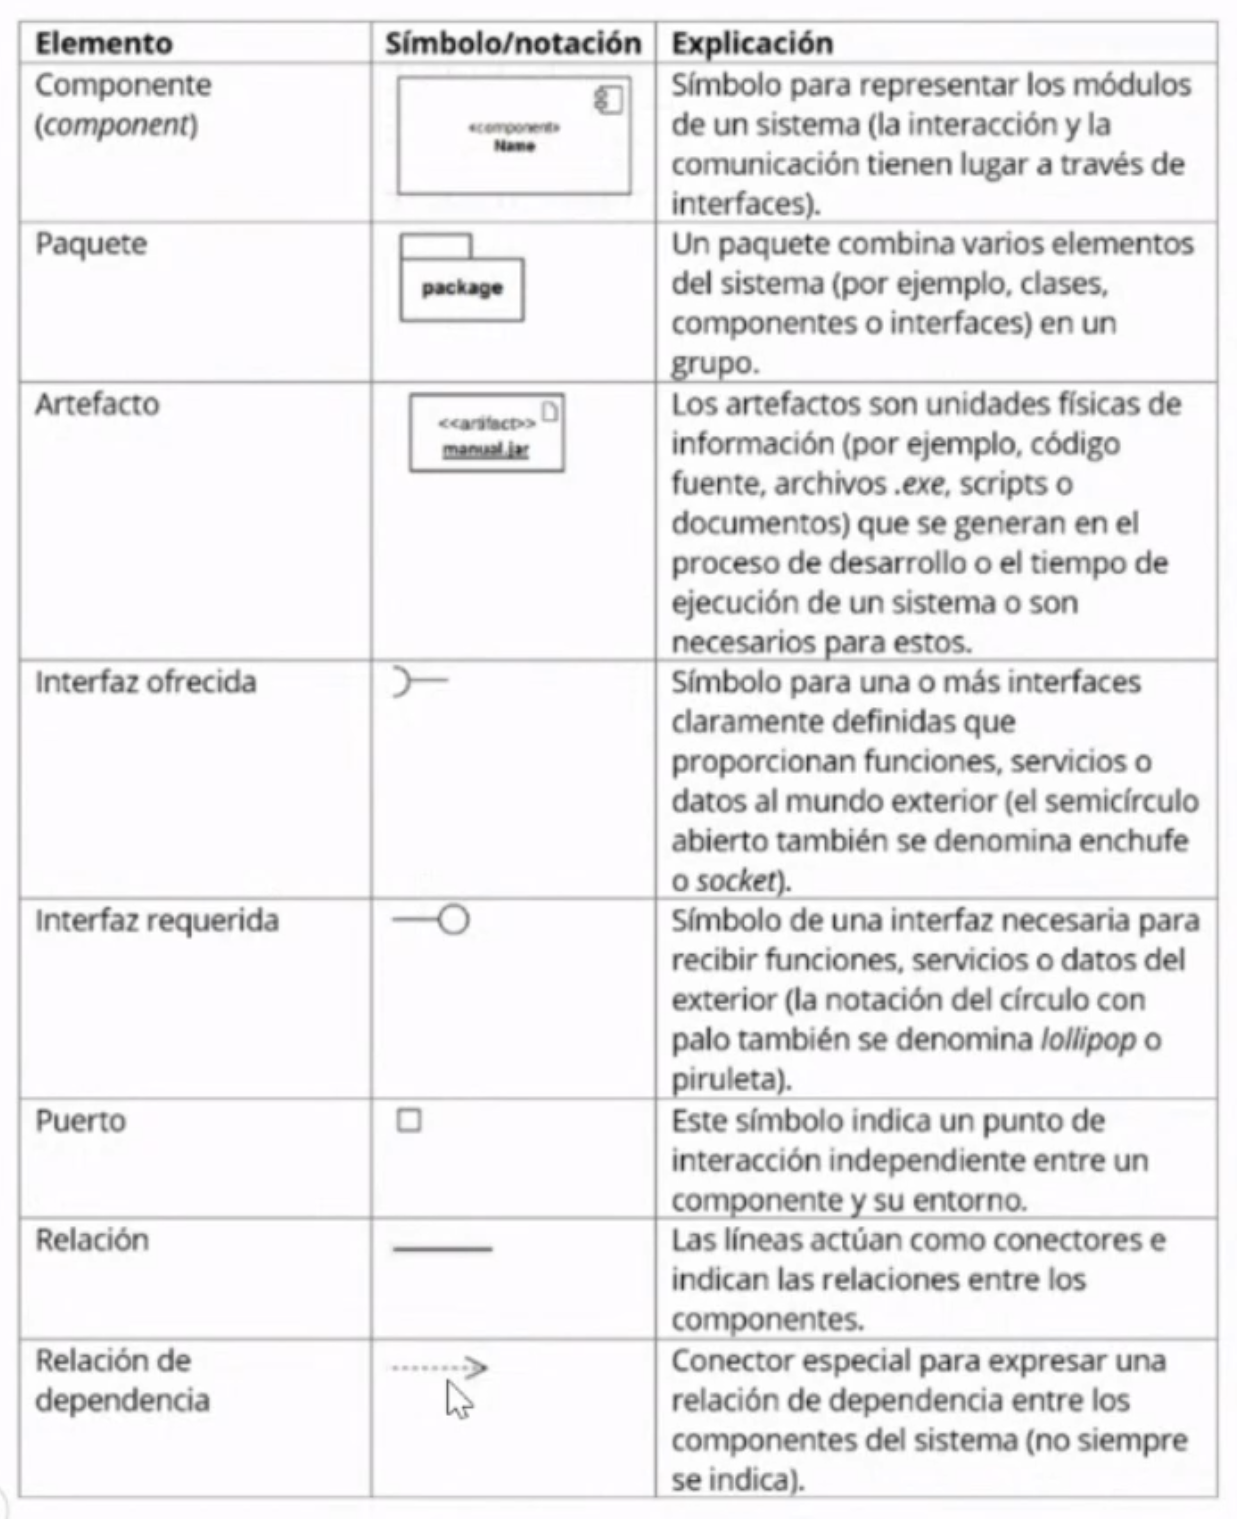
\includegraphics[scale=.25]{Untitled 35.png}}
\end{figure}
\pagebreak
Patrones
\begin{figure}[H]
	\ffigbox[\FBwidth]
	{\caption{Patrones de arquitectura}}
	{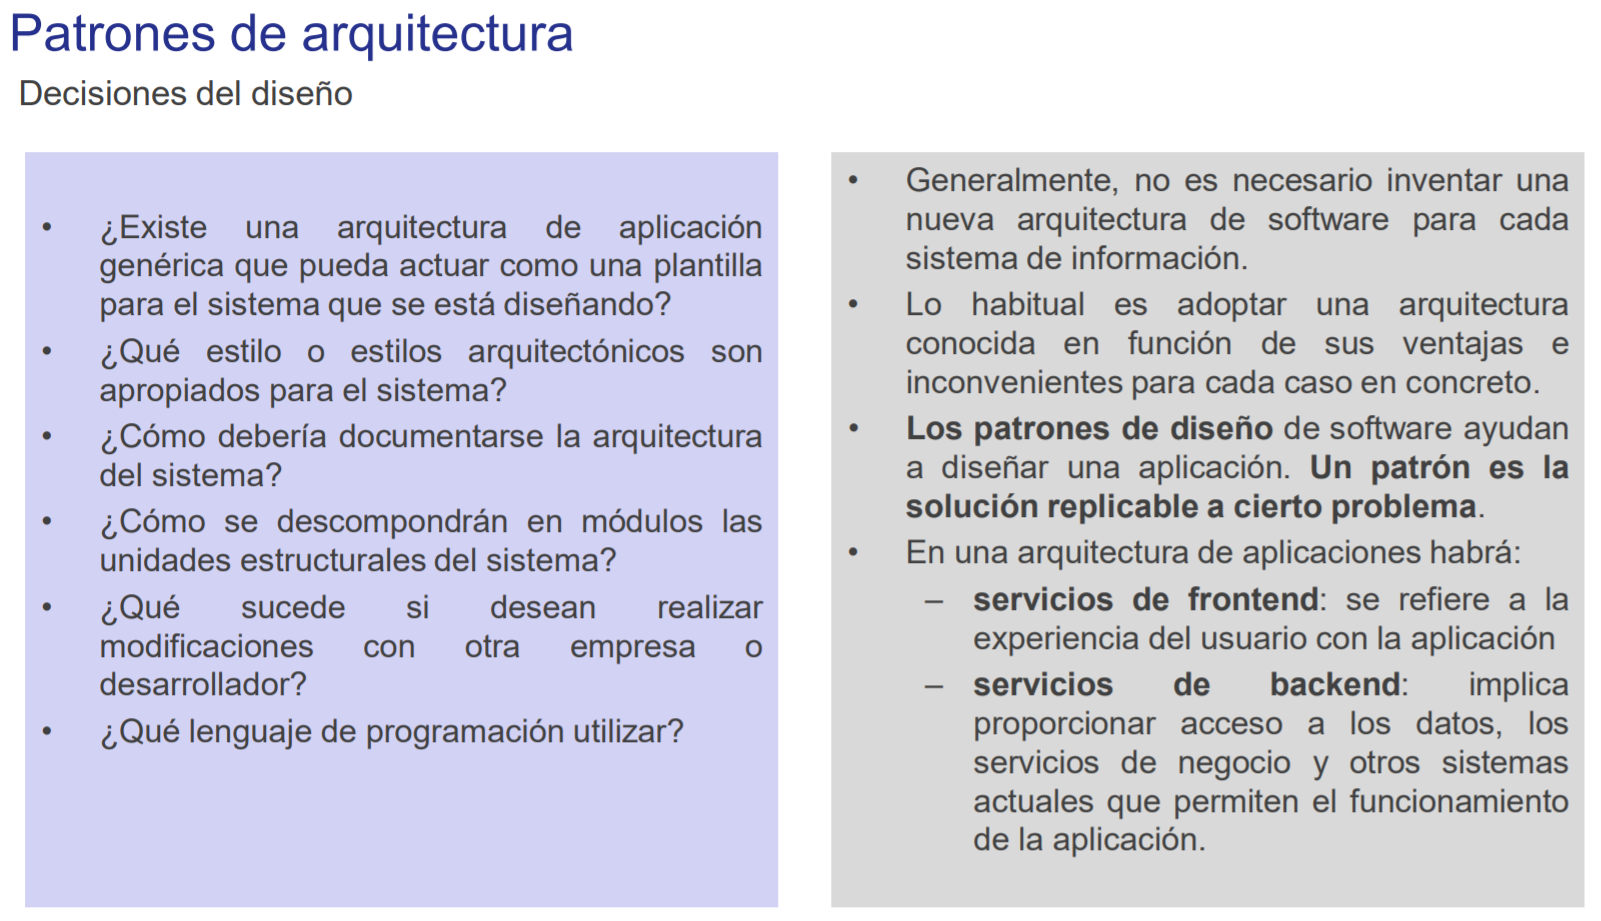
\includegraphics[scale=.25]{Untitled 37.png}}
\end{figure}
\begin{itemize}
	\item Monolito
		\begin{itemize}
			\item
				Los monolitos son otro tipo de arquitectura asociado con los
				sistemas heredados.
			\item
				Antes las aplicaciones se escribían como una sola unidad de
				código, en la que todos los elementos compartían los mismos
				recursos y espacio de memoria.
			\item
				Son pilas de aplicaciones únicas que contienen todas las funciones
				dentro de cada aplicación. Tienen conexión directa, tanto en la
				interacción entre los servicios como en la manera en que se
				desarrollan y distribuyen.
			\item
				Esto implica que al actualizar o ampliar un solo aspecto de una
				aplicación monolítica, habrá una repercusión en toda esa
				aplicación y en la infraestructura subyacente.
		\end{itemize}
	\item Cliente-servidor
		\begin{itemize}
			\item Donde el software reparte su carga de cómputo en dos partes
				independientes, pero sin reparto claro de funciones.
		\end{itemize}
	\item Modelo Vista Controlador
		\begin{itemize}
			\item Es el conocido MVC, que divide una aplicación interactiva en tres
				partes (modelo, vista, controlador) encargadas de contener la
				funcionalidad, mostrar la información al usuario y manejar su
				entrada. Este patrón de arquitectura de software separa los datos
				y la lógica de negocio de una aplicación de su representación.
					\begin{itemize}
						\item
						El Modelo: Es la representación de la información con la cual el
						sistema opera, por lo tanto, gestiona todos los accesos a dicha
						información, tanto consultas como actualizaciones, implementando
						también los privilegios de acceso que se hayan descrito en las
						especificaciones de la aplicación (lógica de negocio). En los
						frameworks actuales normalmente representa una entidad del
						diagrama entidad-relación.
						\item
						La Vista: presenta el modelo (información y lógica de negocio)
						en un formato adecuado para que un usuario pueda interactuar
						(usualmente la interfaz de usuario).
						\item
						El controlador: es el intermediario entre la vista y el modelo,
						su función consiste en controlar el flujo de datos, responder a
						eventos (usualmente provocados por los usuarios) e invocar
						peticiones al modelo.
					\end{itemize}
			\item Maestro esclavo
				\begin{itemize}
					\item Suele utilizarse para replicaciones en la base de datos (la
					maestra es la fuente autorizada y las esclavas se sincronizan
					con ella). Estas dos partes distribuyen el trabajo y calculan el
					resultado final de toda la actividad que realizan dichos
					esclavos. Este patrón es una arquitectura fundamental que los
					desarrolladores utilizan cuando tienen dos o más procesos que
					necesitan ejecutarse de forma simultánea.
				\end{itemize}
			\item Igual a igual (pares)
				\begin{itemize}
					\item Todos los elementos individuales se les denomina `pares', que
					pueden funcionar tanto como `cliente', como `servidor'. Además,
					pueden ir cambiando su rol con el paso del tiempo.
				\end{itemize}
			\item En tuberías
				\begin{itemize}
					\item Arquitecturas de flujo de datos. Esta arquitectura se aplica
					cuando los datos de entrada son transformados a través de una
					serie de componentes computacionales o manipulativos en los
					datos de salida. Típicamente usada en procesamiento de señales y
					transformación de flujos de datos. Los componentes reciben el
					nombre de `filtros' conectados entre sí por `tuberías' que
					transmiten los datos.
				\end{itemize}
			\item En pizarra
			\item Es una arquitectura centradas de datos. Algunas veces llamado
				Blackboard. En el centro de esta arquitectura se encuentra un
				almacén de datos (por ejemplo, un documento o una base de datos)
				al que otros componentes acceden con frecuencia para actualizar,
				añadir, borrar o bien modificar los datos del almacén. Muy
				utilizada en sistemas expertos, visión artificial, interpretación
				sensorial.
		\end{itemize}
\end{itemize}
\pagebreak
Interfaz: Manera de comunicarse entre los componentes.
\begin{itemize}
	\item Conjunto de operaciones que requiere u ofrece un componente.
	\item Manera en la que un componente se comunica con el exterior u
		ofrecer nuestros servicios el sistema.
	\item No necesariamente el flujo de información ofrecida ha recorrido.
	\item Toda manera de intercambiar información del sistema. Ejem:
		Botones, pilotitos, enviar datos\ldots{}
		\begin{itemize}
			\item Un componente puede ofrecer más de una interfaz.
			\item Una interfaz puede ser ofrecida por más de un componente.
		\end{itemize}
	\item Encapsulamiento: Separación de la interfaz y la implementación.
		\begin{itemize}
			\item Una clase/componente puede realizar una o varias interfaces.
			\item Una interfaz puede ser realizada por una o varias clases.
			\begin{figure}[H]
				\ffigbox[\FBwidth]
				{\caption{Encapsulamiento}}
				{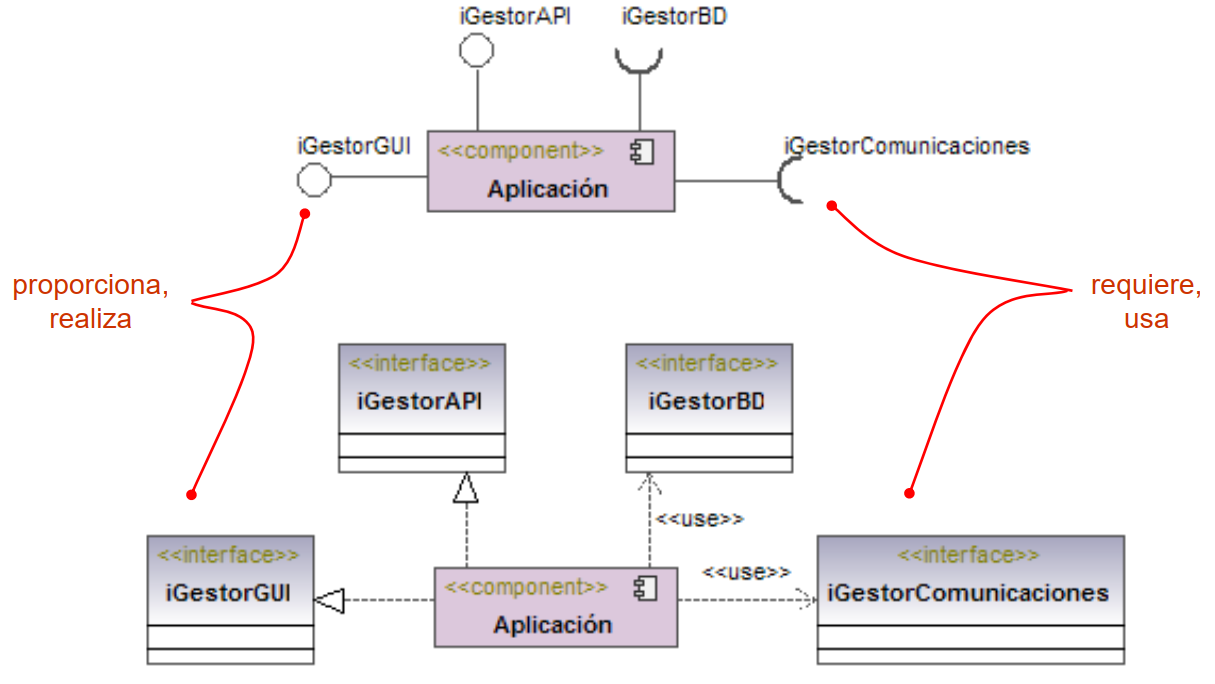
\includegraphics[scale=.3]{Untitled 43.png}}
			\end{figure}
		\end{itemize}
	\item Conjunto de operaciones que ofrecen un servicio coherente:
		\begin{itemize}
			\item no contiene la implementación de las operaciones.
			\item una interfaz no puede tener atributos ni asociaciones.
			\item analogía a una clase abstracta con todas sus operaciones
			abstractas: no puede tener instancias directas.
		\end{itemize}
\end{itemize}
\pagebreak
	Diseño por contratos: Acuerdo entre partes.

    \begin{itemize}
    
    \item
      Condiciones a cumplir entre las interfaces de componentes.
    \item
      Se busca que los componentes y sus relaciones sean
      seguras/robustas.
    \item
      Busca la robustez y corrección.
    \item
      Precondición: Condiciones que debe cumplir las interfaces
      requeridas. Inquilino.
    \item
      Postcondición: Condición que debe cumplir las interfaces
      ofrecidas. Propietario.
    \item
      Contrato: Documento que describe qué es lo que se espera de un
      sistema, enfatizando más en el análisis que en el diseño, más en
      el qué que en el cómo. Lo más común es en forma pre y post.
      Describe el comportamiento esperado del sistema en cada operación.
    \item
      Programación defensiva a errores vs Diseño por contratos:

      \begin{itemize}
      
      \item
        Programación defensiva a errores: Se distribuyen los componentes
        en distintos equipos de programación sin coordinación entre
        ellos, lo que provoca que haya redundancias que en conjunto haya
        más errores, es más difícil de entender en conjunto. Cada uno se
        protege del siguiente, hay más redundancia y devuelve más
        difícil.
      \item
        Diseño por contratos: La aproximación de diseño por contrato es
        mucho mejor que la programación defensiva, se ponen pre y post
        condiciones en cada parte y de esta manera están más
        coordinados. Están más acotadas las funciones y los límites
        entre componentes.
      \end{itemize}
    \item
      Cliente y proveedor acuerdan un contrato.
    \item
      Semántica:

      \begin{itemize}
      
      \item
        Precondiciones: Cliente debe asegurarse de que se cumple.
        Proveedor comprueba.
      \item
        Postcondiciones: Proveedor debe asegurarse de que se cumple. Lo
        que el cliente espera del servidor.
      \item
        Invariantes: Aserción que deben ser ciertas en todo momento.

        \begin{itemize}
        
        \item
          Las operaciones pueden violarlos temporalmente y de modo
          controlado durante su ejecución.
        \item
          La violación de un invariante es un error grave.
        \end{itemize}
      \end{itemize}
	\pagebreak
    \item
      Herencia:

      \begin{itemize}
      
      \item
        Superclase subcontrata a las subclases para las instancias
        directas de la subclase.
      \item
        Las instancias de la subclase son también instancias de la
        superclase.
      \item
        Las invariantes pueden ser más restrictivo en la subclase, pero
        no menos restrictivo.
      \item
        Regla o principio de subcontratación: la operación redefinida en
        una subclase debe\ldots{}

        \begin{itemize}
			\item
			debilitar o mantener la precondición.
			\item
			reforzar o mantener la postcondición.
        \end{itemize}
      
      \end{itemize}
    \end{itemize}

	Ejemplo:
	\begin{figure}[H]
		\ffigbox[\FBwidth]
		{\caption{Ejemplo diagrama de componentes}}
		{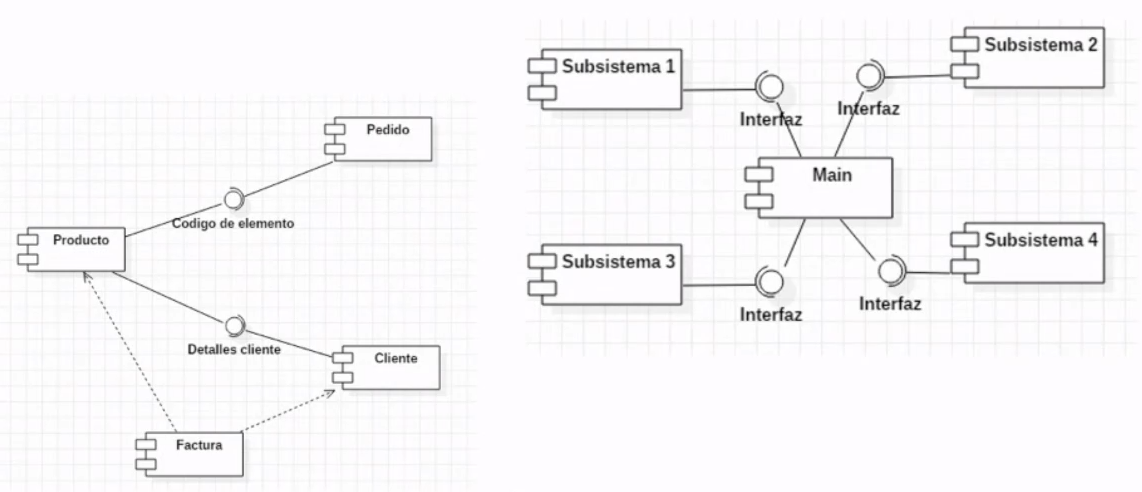
\includegraphics[scale=.3]{Untitled 44.png}}
	\end{figure}



\part{Práctica}
  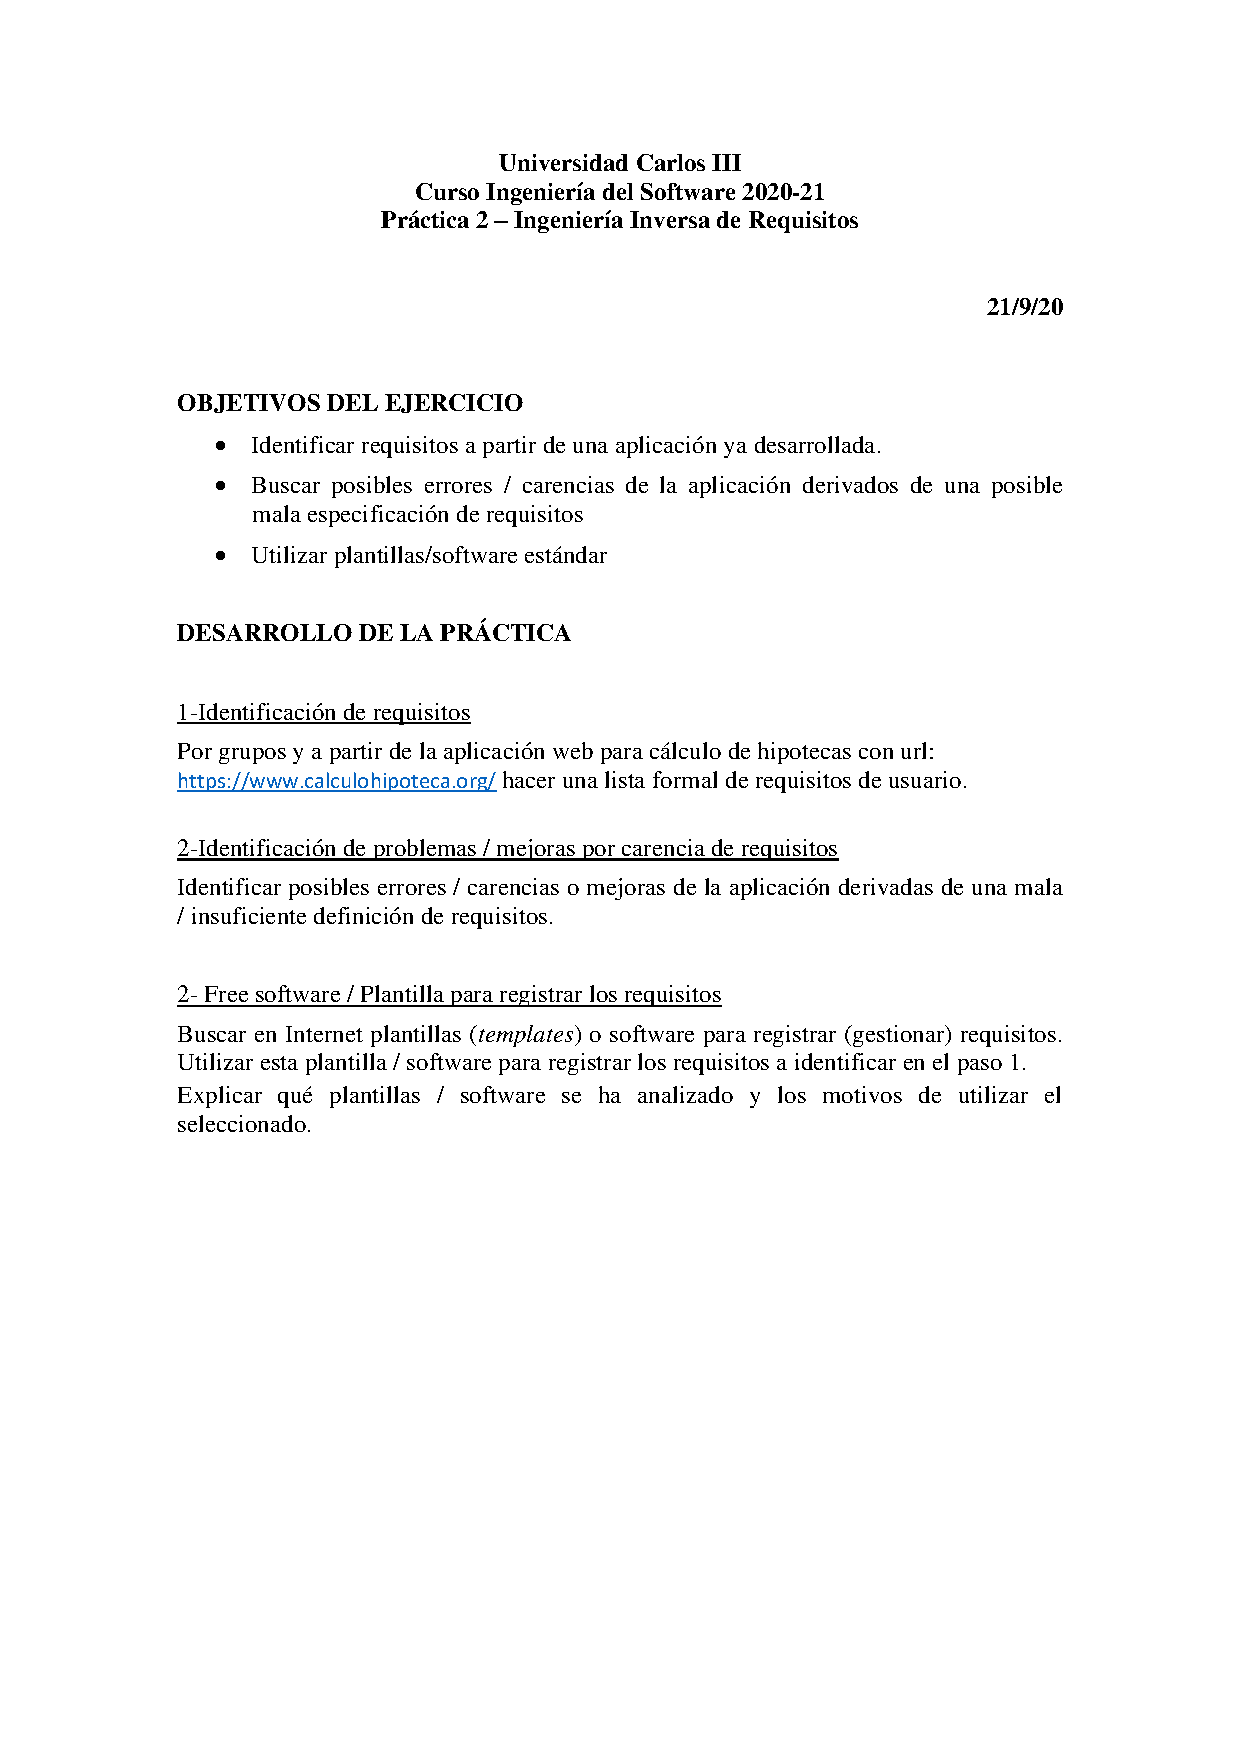
\includepdf[pages=-]{docs/Practica_2_-_Ingenieria_Inversa.pdf}
  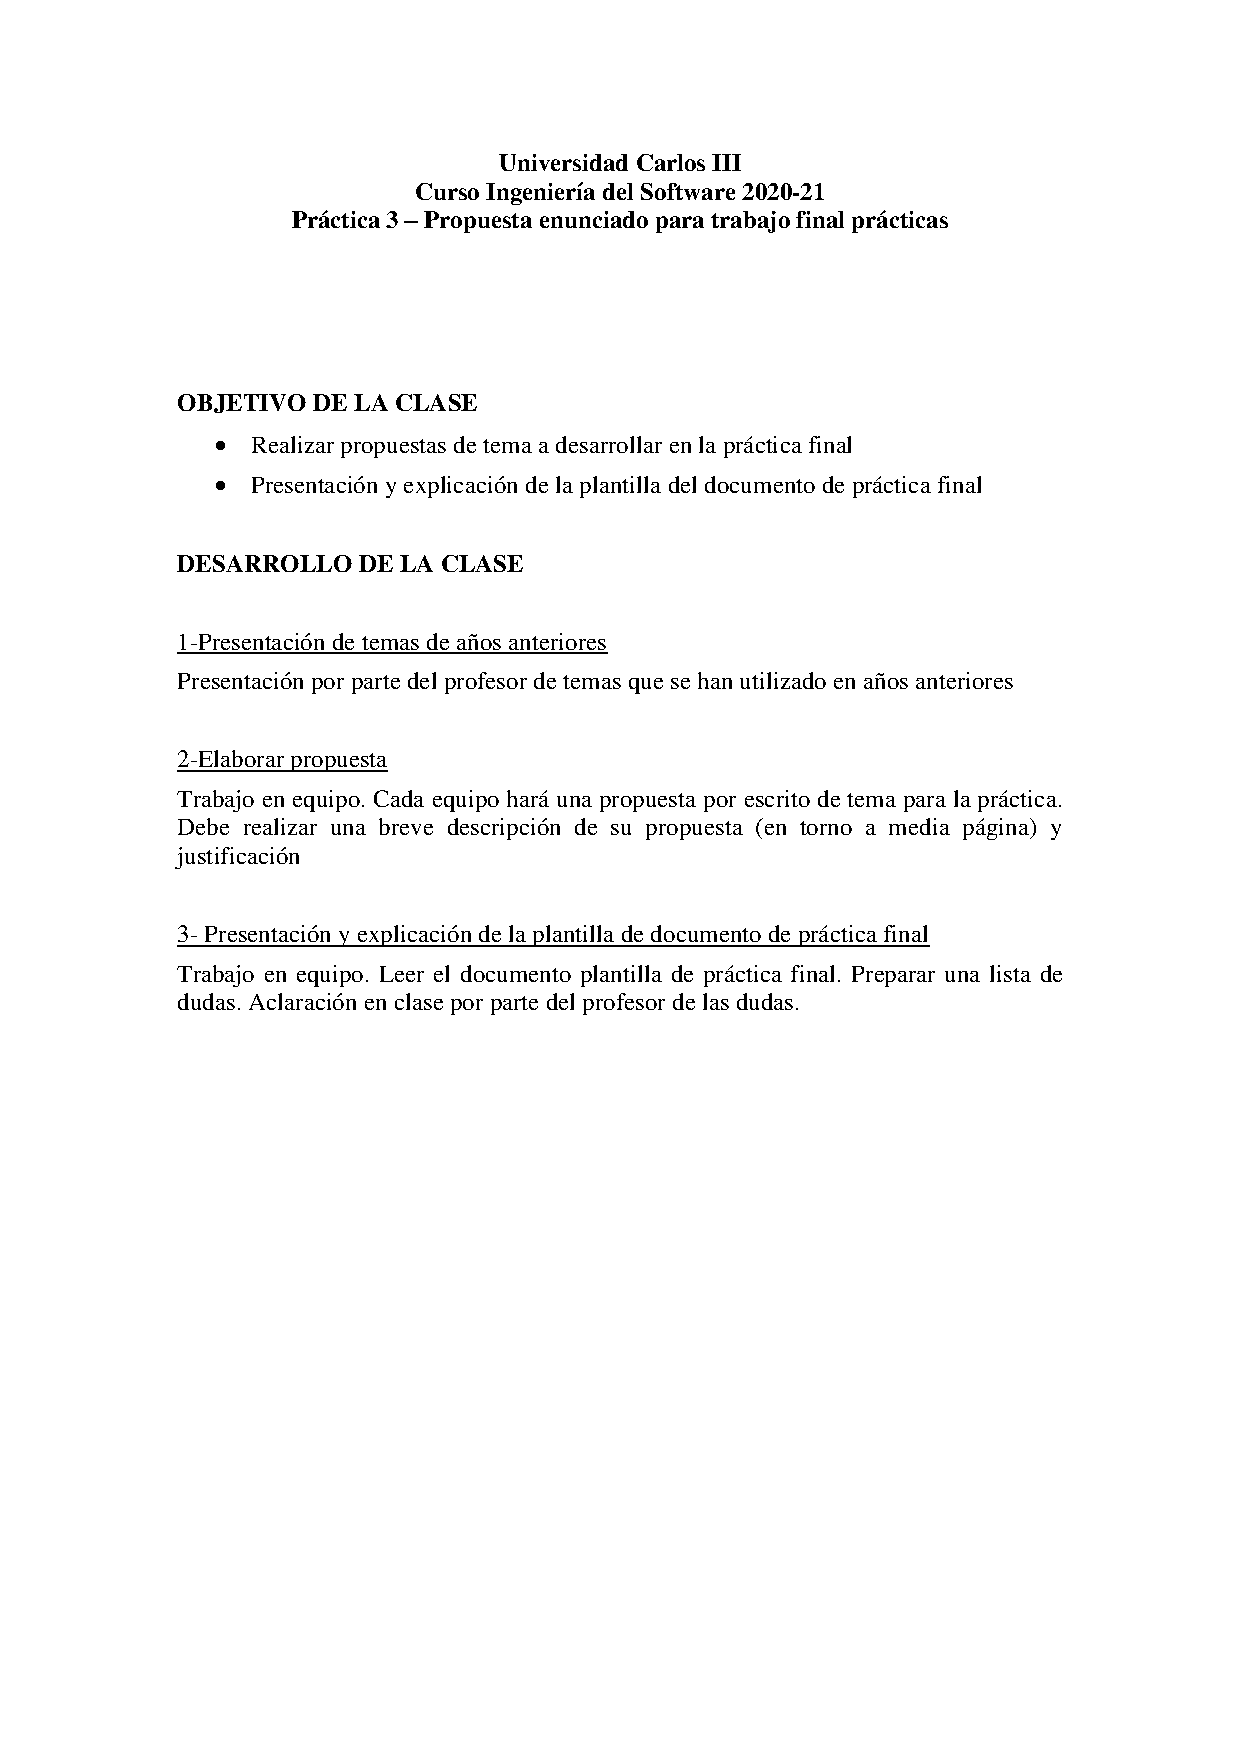
\includepdf[pages=-]{docs/Practica_3_-_Propuesta_Enunciado.pdf}
  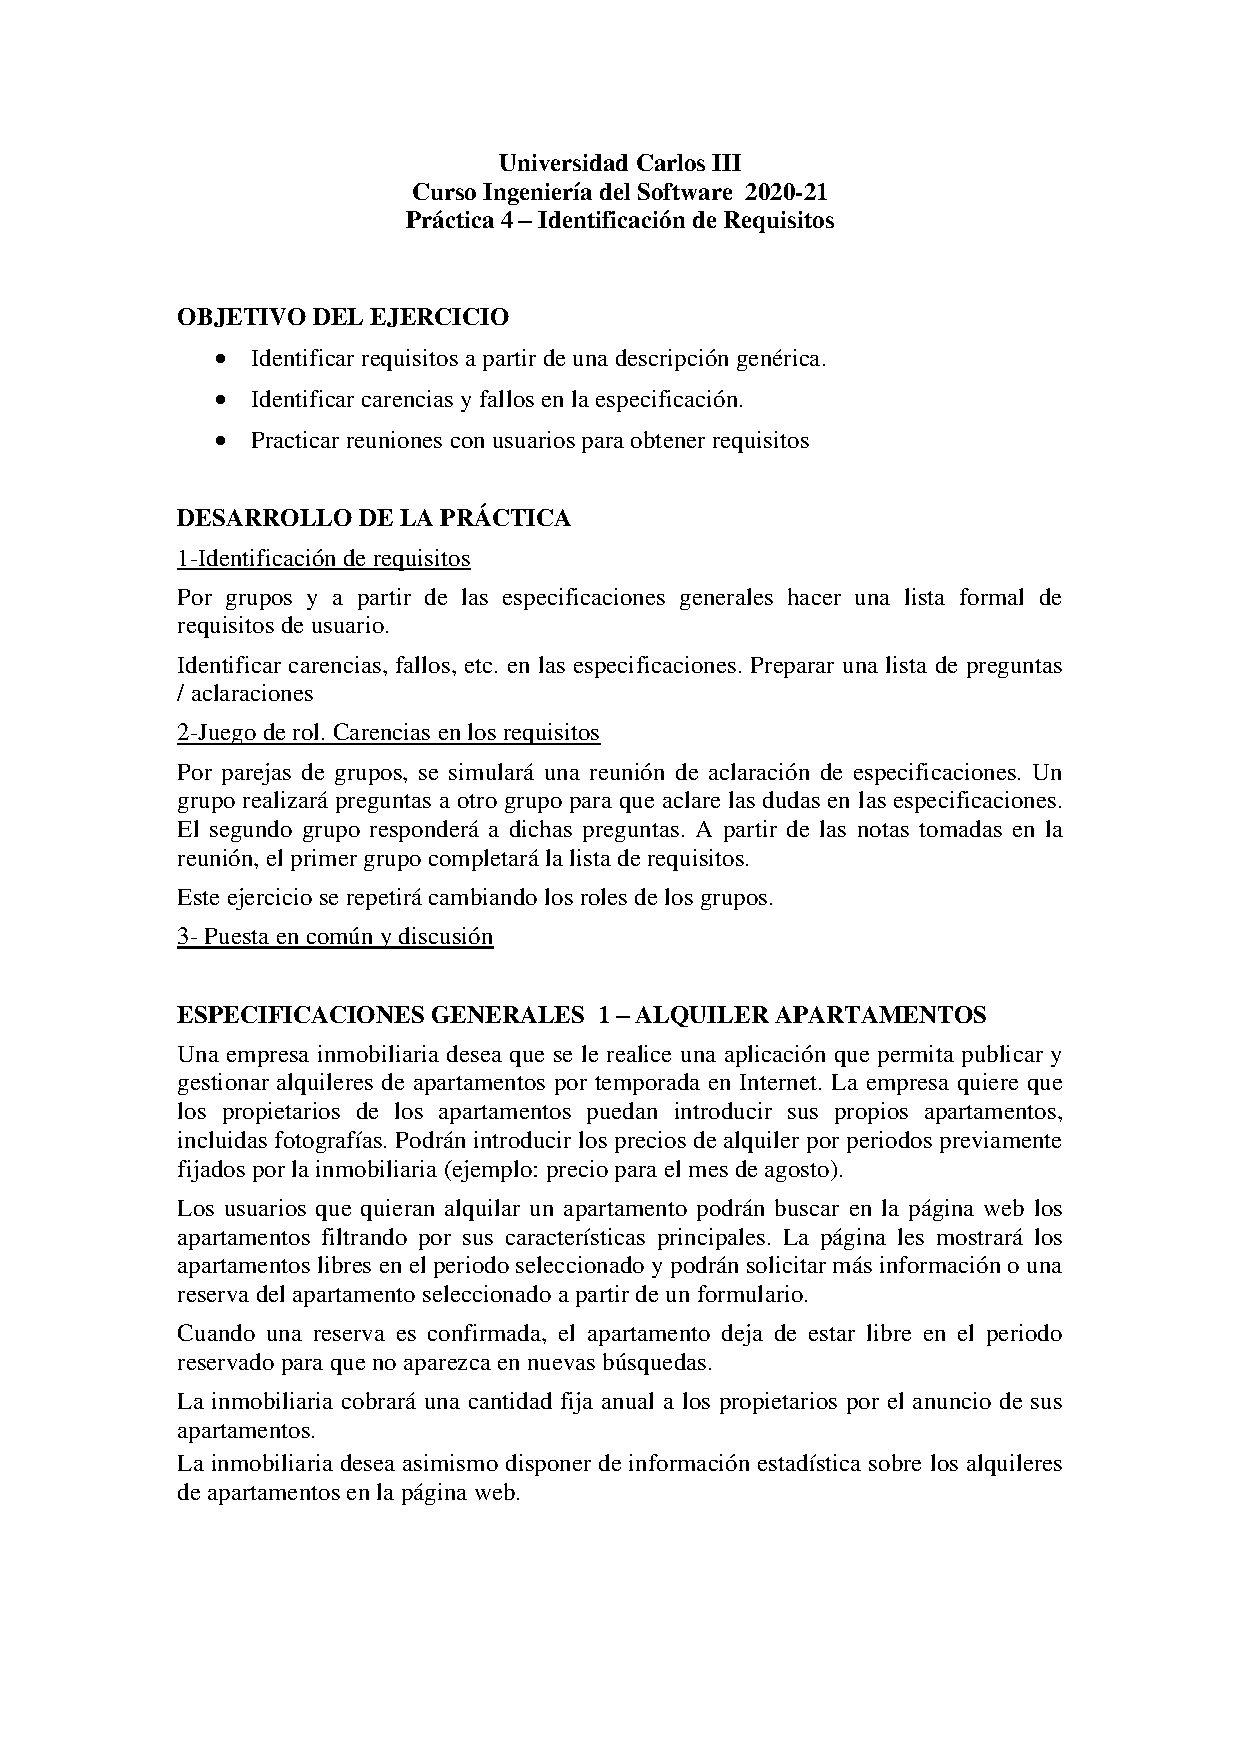
\includepdf[pages=-]{docs/Practica_4_-_Identificacion_de_Requisitos.pdf}
  \includepdf[pages=-]{docs/Practica_5_-_Errores_en_Requisitos.pdf}
  \includepdf[pages=-]{docs/Practica_6_y_7_-_Modelado_conceptual.pdf}
  
\includepdf[pages=-]{docs/Prctica_8_-_Preparacin_ejercicio.pdf}
  
\includepdf[pages=-]{docs/IS_2021_Plantilla_Prctica_1.pdf}
  \includepdf[pages=-]{docs/IS_2021_Plantilla_Prctica_Entrega_2.pdf}
  \includepdf[pages=-]{docs/Entrega3ProyectoFinalGrupo9.pdf}
  \includepdf[pages=-]{docs/PreguntasIS-T09.pdf}
  \includepdf[pages=-]{docs/IS_2021_Revisin_por_pares.pdf}
  \includepdf[pages=-]{docs/Anexo_Requisitos_.pdf}
  
\includepdf[pages=-]{docs/181-09_Entrega_final.pdf}
  \includepdf[pages=-]{docs/Anexo_I.pdf}
  \includepdf[pages=-]{docs/Anexo_II.pdf}
  \includepdf[pages=-]{docs/Anexo_III.pdf}

\end{document}